% SIAM Article Template
\documentclass[review,onefignum,onetabnum]{siamonline220329}

% Information that is shared between the article and the supplement
% (title and author information, macros, packages, etc.) goes into
% ex_shared.tex. If there is no supplement, this file can be included
% directly.

% SIAM Shared Information Template
\documentclass[preprint,onefignum,onetabnum]{siamart220329}

% This is information that is shared between the main document and any
% supplement. If no supplement is required, then this information can
% be included directly in the main document.


% Packages and macros go here
\usepackage{lipsum}
\usepackage{amssymb}
\usepackage{amsfonts}
\usepackage{graphicx}
\usepackage{epstopdf}
\usepackage{algorithmic}
\usepackage{tikz}
\usepackage{pgfplots}
\usetikzlibrary{shapes.arrows, patterns, calc}
\usepackage{tikz-3dplot}
\usepackage{bbm}
\usepackage{bm}
\ifpdf
  \DeclareGraphicsExtensions{.eps,.pdf,.png,.jpg}
\else
  \DeclareGraphicsExtensions{.eps}
\fi
\usepackage{todonotes}

\definecolor{lightblue}{HTML}{a1b4c7}
\definecolor{orange}{HTML}{ea8810}
\definecolor{silver}{HTML}{b0aba8}
\definecolor{rust}{HTML}{b8420f}
\definecolor{seagreen}{HTML}{23553c}

\colorlet{lightsilver}{silver!30!white}
\colorlet{darkorange}{orange!85!black}
\colorlet{darksilver}{silver!85!black}
\colorlet{darklightblue}{lightblue!85!black}
\colorlet{darkrust}{rust!85!black}
\colorlet{darkseagreen}{seagreen!85!black}

\hypersetup{
  colorlinks=true,
  linkcolor=darkrust,
  citecolor=darkseagreen,
  urlcolor=darksilver
}

\pgfplotsset{compat=newest}
\usepgfplotslibrary{fillbetween}

% custom commands:
% \newcommand{\todo}[1]{{\color{red} #1}}
\newcommand{\Ftodo}[1]{\todo[color=lightblue]{Florian: #1}}
\newcommand{\Stodo}[1]{\todo[color=seagreen]{Stephen: #1}}

\usepackage{mathtools}
%Names of standard objects
\newcommand*{\Reals}{\mathbb{R}}
\newcommand*{\Naturals}{\mathbb{N}}

\makeatletter
\renewcommand{\paragraph}{%
  \@startsection{paragraph}{4}%
  {\z@}{1.0ex \@plus .5ex \@minus .2ex}{-.7em}%
  {\normalfont\normalsize\bfseries}%
}
\makeatother

% From https://tex.stackexchange.com/questions/198771/align-in-substack
\makeatletter
\newcommand{\subalign}[1]{%
  \vcenter{%
    \Let@ \restore@math@cr \default@tag
    \baselineskip\fontdimen10 \scriptfont\tw@
    \advance\baselineskip\fontdimen12 \scriptfont\tw@
    \lineskip\thr@@\fontdimen8 \scriptfont\thr@@
    \lineskiplimit\lineskip
    \ialign{\hfil$\m@th\scriptstyle##$&$\m@th\scriptstyle{}##$\hfil\crcr
      #1\crcr
    }%
  }%
}
\makeatother

%Names of Variables:
\newcommand*{\stateP}{\mathbf{x}}
\newcommand*{\stateD}{\hat{\mathbf{x}}}

\newcommand*{\resP}{\mathbf{r}}
\newcommand*{\resD}{\hat{\mathbf{r}}}

\newcommand*{\resMatP}{\mathbf{R}}
\newcommand*{\resMatD}{\hat{\mathbf{R}}}


\newcommand*{\dirP}{\mathbf{p}}
\newcommand*{\dirMatP}{\mathbf{P}}
\newcommand*{\dirD}{\hat{\mathbf{p}}}
\newcommand*{\dirMatD}{\hat{\mathbf{P}}}

\newcommand*{\rhsP}{\mathbf{b}}
\newcommand*{\rhsD}{\hat{\mathbf{b}}}

\newcommand*{\mat}{\mathbf{A}}
\newcommand*{\adj}[1]{#1^{\dagger}}
\newcommand*{\con}[1]{\bar{#1}}

\newcommand*{\alphaP}{\alpha}
\newcommand*{\alphaD}{\hat{\alpha}}

\newcommand*{\alphaMatP}{\bm{\alpha}}
\newcommand*{\alphaMatD}{\hat{\bm{\alpha}}}

\newcommand*{\betaP}{\beta}
\newcommand*{\betaD}{\hat{\beta}}

\newcommand*{\betaMatP}{\bm{\beta}}
\newcommand*{\betaMatD}{\hat{\bm{\beta}}}

\renewcommand{\vec}[1]{\bm{#1}}

\renewcommand{\algorithmicrequire}{\textbf{Input:}}
\renewcommand{\algorithmicensure}{\textbf{Output:}}

% Add a serial/Oxford comma by default.
\newcommand{\creflastconjunction}{, and~}

% Used for creating new theorem and remark environments
\newsiamremark{remark}{Remark}
\newsiamremark{hypothesis}{Hypothesis}
\newsiamremark{example}{Example}
\crefname{hypothesis}{Hypothesis}{Hypotheses}
\newsiamthm{claim}{Claim}

% Sets running headers as well as PDF title and authors
\headers{Factorization by greedy conditional selection}{
S. Huan, J. Guinness, M. Katzfuss, H. Owhadi, F. Sch{\"a}fer}

% Title. If the supplement option is on, then "Supplementary Material"
% is automatically inserted before the title.
\title{Sparse Cholesky factorization by greedy conditional selection}

% Authors: full names plus addresses.
\author{
  Stephen\ Huan\thanks{Georgia Institute of Technology} \and
  Joe\ Guinness\thanks{Joe} \and
  Matthias\ Katzfuss\thanks{Matthias} \and
  Houman\ Owhadi\thanks{Houman} \and
  Florian\ Sch{\"a}fer\thanks{Georgia Institute of Technology,
  S1317 CODA, 756 W Peachtree St Atlanta, GA 30332, \newline
  \email{florian.schaefer@cc.gatech.edu},\newline Corresponding Author}
}


\usepackage{amsopn}
\DeclareMathOperator{\diag}{diag}
\let\trace\relax
\DeclareMathOperator{\trace}{trace}
\DeclareMathOperator{\logdet}{logdet}
\DeclareMathOperator{\chol}{chol}

\DeclareMathOperator*{\argmin}{argmin}

\DeclareMathOperator{\E}{E}
\DeclareMathOperator{\Var}{Var}
\DeclareMathOperator{\Cov}{Cov}
\DeclareMathOperator{\Corr}{Corr}
\DeclareMathOperator{\I}{MI}
\DeclareMathOperator{\entropy}{H}

%%% Local Variables:
%%% mode:latex
%%% TeX-master: "ex_article"
%%% End:


% Optional PDF information
\ifpdf
\hypersetup{
  pdftitle={Sparse Cholesky factorization by greedy conditional selection},
  pdfauthor={S. Huan, J. Guinness, M. Katzfuss, H. Owhadi, F. Sch{\"a}fer}
}
\fi

% The next statement enables references to information in the
% supplement. See the xr-hyperref package for details.

\externaldocument{experimental_design_linalg_supplement}

% FundRef data to be entered by SIAM
%<funding-group specific-use="FundRef">
%<award-group>
%<funding-source>
%<named-content content-type="funder-name">
%</named-content>
%<named-content content-type="funder-identifier">
%</named-content>
%</funding-source>
%<award-id> </award-id>https://www.overleaf.com/project/62db5b8df06c896e5b905c30
%</award-group>
%</funding-group>

\begin{document}

\maketitle

% REQUIRED
\begin{abstract}
  Dense kernel matrices resulting from pairwise evaluations of a
  kernel function arise naturally in machine learning and statistics.
  Previous work in constructing sparse transport maps or sparse approximate
  inverse Cholesky factors of such matrices by minimizing Kullback-Leibler
  divergence recovers the Vecchia approximation for Gaussian processes.
  These methods rely only on the geometry of the
  evaluation points to construct the sparsity pattern.
  In this work, we instead construct the sparsity pattern by leveraging
  a greedy selection algorithm that maximizes mutual information
  with target points, conditional on all points previously selected.
  For selecting \( k \) points out of \( N \), the naive time
  complexity is \( \mathcal{O}(N k^4) \), but by maintaining a
  partial Cholesky factor we reduce this to \( \mathcal{O}(N k^2) \).
  Furthermore, for multiple (\( m \)) targets we achieve a time complexity of
  \( \mathcal{O}(N k^2 + N m^2 + m^3) \) which is maintained in the setting of
  aggregated Cholesky factorization where a selected point need not condition
  every target.
  We apply the selection algorithm to image
  classification and recovery of sparse Cholesky factors.
  By minimizing Kullback-Leibler divergence, we apply the algorithm to Cholesky
  factorization, Gaussian process regression, and preconditioning with the
  conjugate gradient, improving over \( k \)-nearest neighbors particularly in
  high dimensional, unusual, or otherwise messy geometries.
\end{abstract}

% REQUIRED
\begin{keywords}
  \todo{to do}
\end{keywords}

% REQUIRED
\begin{AMS}
  % 68Q25, 68R10, 68U05
\end{AMS}

\section{Introduction}

\paragraph{The problem}

Gaussian processes are widely used in spatial statistics
and geostatistics \cite{rue2005gaussian}, machine learning
through kernel methods \cite{rasmussen2006gaussian}, optimal
experimental design \cite{mutny2022experimental}, and sensor
placement \cite{krause2008nearoptimal}.
Applying Gaussian process statistics to sets of \( N \) data
points requires computing with the covariance matrix \( \CM
\in \Reals^{N \times N} \) to obtain quantities such as \(
\CM \vec{v} \), \( \CM^{-1} \vec{v} \), \( \logdet(\CM) \).
For dense \( \CM \), directly computing these quantities has a
computational cost of \( \BigO(N^3) \) and a memory cost of \(
\BigO(N^2) \), which is prohibitively expensive for large \( N \).
Beyond Gaussian processes, computations with large positive-definite
matrices are required across computational mathematics,
motivating the search for faster, approximate algorithms.

\paragraph{Existing work}

Numerous methods have been proposed for fast
approximate Gaussian process statistics.
Popular methods are based on low-rank approximation \cite{smola2000sparse,
williams2000using, fine2001efficient, bach2002kernel, fowlkes2004spectral,
chen2022randomly}, sparse approximations \cite{furrer2006covariance},
or combinations thereof \cite{schwaighofer2002transductive,
quinonero-candela2005unifying, banerjee2008gaussian, sang2012full}.
These approximations can be viewed as imposing different
(conditional) independence structures on the Gaussian process.
Multiscale-versions of these ideas lead to wavelets \cite{beylkin1991fast,
gines1998lu} and various structured matrix factorizations
\cite{hackbusch2000sparse, hackbusch2002data, chandrasekaran2006fast,
xia2010fast, li2012new, ambikasaran2013mathcal, ambikasaran2015fast,
ho2016hierarchical, schafer2020compression}.
Alternatives are based on fast Fourier
transforms \cite{graham2018analysis, stein2002fast}
or random feature maps \cite{rahimi2007random}.

\paragraph{Vecchia approximation, Kaporin's factorization, and KL minimization}

Vecchia approximates the likelihood function of a Gaussian
distribution by decomposing it into a product of univariate
conditional densities, each of which depends on a subset of
the previous variables \cite{vecchia1988estimation}.
Independently from Vecchia, Kaporin derived a closed-form expression of
the approximate inverse Cholesky preconditioner of a p.s.d. matrix that
minimizes, subject to a sparsity constraint, the \( K \)-condition number
of the preconditioned system \cite{kaporin1990alternative}.
Referring to this approximation as ``factorized sparse approximate inverse
(FSAI),'' Yeremin et al. show that Kaporin's inverse Cholesky factor also
minimizes a Frobenius-norm error metric, subject to a diagonal scaling
constraint \cite{yeremin2000factorized}.
Vecchia's likelihood approximation was later observed to
implicitly compute a sparse approximate inverse Cholesky
factor of the covariance matrix \cite{katzfuss2021general}.
The closed-form expression of this inverse Cholesky
factor coincides with that derived by Kaporin.
Independently from the above works, Sch{\"a}fer et al. compute sparse inverse
Cholesky factors that are optimal in Kullback-Leibler (KL) divergence
\cite{schafer2021sparse}, again recovering the formula derived by Kaporin.
The KL divergence is also used to compute Knothe-Rosenblatt transport
maps \cite{marzouk2016introduction}, generalizing Cholesky factors to
non-Gaussian distributions while preserving triangularity and sparsity
\cite{spantini2018inference}.
A method for the Bayesian estimation of such transport
maps is proposed by \cite{katzfuss2022scalable}.
A common feature of the above methods is that the columns of the
Cholesky factors can be computed independently and in parallel.

\paragraph{Ordering and sparsity selection by geometry}
The approximation quality of the above methods depends on the ordering of the rows and columns of the input matrix and the sparsity pattern of the factor.
Vecchia originally proposed ordering points lexicographically \cite{vecchia1988estimation}. 
The work on FSAI emphasized classical orderings from sparse linear algebra 
such as (reverse) Cuthill-McKee, minimum degree, nested dissection, and red-black ordering \cite{benzi2000orderings}.  
Guinness empirically studied the effect of various orderings on Vecchia's likelihood approximation \cite{guinness2018permutation}.  
He found the random ordering and a space-filling maximum-minimum distance (maximin) ordering to perform well.
This observation can be explained by the \emph{screening effect}, by which conditional on points near the point of interest, far away
points are almost conditionally independent for many popular kernel functions
\cite{stein2002screening, stein20112010} (see \cref{fig:screening}).
Cholesky factorization is closely related to numerical homogenization and operator adapted wavelets \cite{owhadi2019operatoradapted}.
Sch{\"a}fer et al. exploit this connection to prove exponential decay of Cholesky factors of covariance and precision matrices arising from elliptic PDEs, when developed in a multiresolution basis \cite{schafer2020compression}. 
This setting includes the maximin ordering as a simplistic multiresolution basis akin to the ``lazy wavelet'' \cite{sweldens1996lifting} and thus provides a rigorous proof of the screening effect.
The maximin ordering has since been used by \cite{schafer2021sparse, katzfuss2021general, kang2021correlationbased, katzfuss2022scalable}.
Motivated by the screening effect, the sparsity
set is often formed by selecting the closest points by Euclidean distance
\cite{vecchia1988estimation, schafer2020compression, schafer2021sparse,
katzfuss2022scalable}.
To lower the computational cost, different authors have proposed heuristics to analyze the sparsity set and identify opportunities to group similar degrees of freedom into supernodes \cite{stein2004approximating,ferronato2015novel,guinness2018permutation}.
Sch{\"a}fer et al. devise a geometric grouping algorithm that allows to provably compute an \( \epsilon \)-accurate inverse-Cholesky factor in time complexity \( \BigO(N
\log^{2d} (N/\epsilon)) \) using \( \BigO(N \log^{ d} (N/\epsilon)) \)
nonzero entries of the covariance matrix \cite{schafer2021sparse}.
Methods based on the screening effect have improved the 
state-of-the-art for solving elliptic differential and integral equations \cite{schafer2020compression,schafer2021sparse,chen2021multiscale}.
However, selecting the sparsity set only based on distance ignores the possible redundancy of the selected points.
The proposed work addresses this limitation.

\begin{figure}[t]
  \centering
  \begin{tikzpicture}
  \begin{axis}[
      width={0.49\linewidth},
      grid={major},
      xmin=-2, xmax=2, ymin=-2, ymax=2, zmin=-0.1, zmax=1,
    ]
    \addplot3 [only marks, orange]
      table {figures/screening/matern_uncond_points.csv};
    \addplot3 [mesh, lightblue]
      table {figures/screening/matern_uncond.csv};
  \end{axis}
\end{tikzpicture}
%
  \begin{tikzpicture}[baseline]
  \begin{axis}[
    width={0.49\linewidth},
    grid={major},
    xmin=-1.1, xmax=1.1, ymin=-1.1, ymax=1.1, zmin=-0.1, zmax=1,
  ]
  \addplot3 [only marks, orange]
    table {figures/screening/matern_cond_points.csv};
  \addplot3 [mesh, seagreen]
    table {figures/screening/matern_cond.csv};
  \end{axis}
\end{tikzpicture}

  \caption{
    An illustration of the screening effect with the Mat{\'e}rn kernel with
    length scale \( \ell = 1 \) and smoothness \( \nu = 1/2 \).
    The first panel shows the \textcolor{lightblue}{unconditional
    correlation} with the point at (0, 0).
    The second panel shows the \textcolor{seagreen}{conditional correlation}
    after conditioning on the four points in \textcolor{orange}{orange}.
  }
  \label{fig:screening}
\end{figure}

\paragraph{Conditional selection}

Instead of adding points to the sparsity pattern by distance, we propose
greedily selecting points that maximize mutual information with the
point of interest, conditional on all points previously selected.
The machine learning community has long developed similar algorithms that
greedily optimize information-theoretic objectives in the context of
sparse Gaussian process inference \cite{smola2000sparse, herbrich2002fast,
seeger2003fast}.
Similar algorithms have also been developed in the context of
sensor placement \cite{krause2008nearoptimal, clark2018greedy}
and experimental design \cite{mutny2022experimental} where it is
assumed the target phenomenon is modeled by a Gaussian process or
is otherwise linearly dependent on the selected measurements.
However, these works often focus on global approximation of the entire process,
e.g., through sparse approximation of the likelihood or covariance matrix
\cite{liu2020when, chalupka2012framework, quinonero-candela2005unifying}.
In contrast \cite{wada2013gaussian} uses inference \emph{directed} towards
a point of interest, selecting the active (sparsity) set by the kernel
function itself like the later work \cite{kang2021correlationbased};
\cite{gramacy2014local} and the follow-up work \cite{gramacy2015speeding}
use the more sophisticated active learning Cohn (ALC) objective, yielding
an algorithm equivalent to ours for a single point of interest.
Our proposed algorithm can also be viewed as a variant of orthogonal matching
pursuit (OMP) \cite{tropp2007signal, tropp2006algorithms}, a workhorse
algorithm in compressive sensing, which seeks to approximate a target signal
as the sparse linear combination from a given collection of signals.

\paragraph{Main results}

Our main contribution is a selection algorithm that
greedily maximizes mutual information with point(s) of
interest, conditional on all points previously selected.
We use this algorithm to select the sparsity pattern of sparse approximate
Cholesky factors of precision matrices in the KL-minimization framework of
\cite{schafer2021sparse}, improving the approximation accuracy attainable
with a given number of nonzero entries.
Our method extends kernel-based selection \cite{wada2013gaussian,
kang2021correlationbased} to account for conditioning.
It also extends directed Gaussian process regression \cite{gramacy2014local,
gramacy2015speeding} by simultaneously targeting multiple prediction
points and providing a global approximation of the Gaussian process.
For a single target point, naive computation of the
mutual information criterion has time complexity \(
\BigO(N k^4) \) to select \( k \) points out of \( N \).
By maintaining a partial Cholesky factor we
reduce the complexity to \( \BigO(N k^2) \).
We extend the algorithm to maximize mutual information with
\emph{multiple} targets, re-using the same selections across
multiple targets for efficiency while maintaining accuracy.
For \( m \) target points we achieve a time
complexity of \( \BigO(N k^2 + N m^2 + m^3) \).
If \( m \approx k \), this is \( m \) times
faster than the single-target algorithm.
In the setting of aggregated (or supernodal) Cholesky factorization where
the sparsity patterns of multiple columns are determined simultaneously,
a candidate entry may only condition a \emph{subset} of the targets.
By efficient rank-one downdating of Cholesky factors, we capture
this structure at the same time complexity for multiple targets.
Finally, we show how to adaptively determine the number of nonzeros
per column in order to minimize the overall KL divergence by
maintaining a global priority queue shared between all columns.

\paragraph{Outline}

This paper is organized as follows.
In \cref{sec:chol}, we show how minimizing KL divergence to compute sparse
Cholesky factors reduces to solving independent regression problems.
In \cref{sec:select}, we develop greedy algorithms to select
the sparsity pattern independently for each regression problem.
In \cref{sec:chol_select}, we combine the greedy selection algorithm with
KL minimization to yield algorithms for sparse Cholesky factorization.
In \cref{sec:extensions} we extend these results to
adjacent and nonadjacent aggregated factorization.
In \cref{sec:experiments}, we present numerical experiments applying
our method to Cholesky factorization, Gaussian process regression,
preconditioning with the conjugate gradient, image classification,
and recovery of \textit{a priori} sparse Cholesky factors.
In \cref{sec:conclusion}, we summarize our results.
Proofs and algorithmic details are provided
in the appendix and supplementary material.

\begin{figure}[t]
  \centering
  % \begin{tikzpicture}[baseline]
  \begin{axis}[
    width={0.25\linewidth},
    height={0.25\linewidth},
    axis lines={none},
    scale only axis=true,
    % legend entries={{}, \( k \)-NN},
    % legend pos={north east},
    legend style={at={(0.9, 0.9)}, anchor=north east},
  ]
  \addplot [only marks, mark size=0.6, silver]   table
    {figures/kernel/grid_1e-5/points.csv};
  \addplot [only marks, mark size=0.6, seagreen] table
    {figures/kernel/grid_1e-5/selected_1.csv};
  \addplot [only marks, mark size=0.6, orange]   table
    {figures/kernel/grid_1e-5/target.csv};
  \end{axis}
\end{tikzpicture}
%
  % \begin{tikzpicture}[baseline]
  \begin{axis}[
    width={0.25\linewidth},
    height={0.25\linewidth},
    axis lines={none},
    scale only axis=true,
    % legend entries={{}, \( \nu = \frac{1}{2} \)},
    % legend pos={north east},
    legend style={at={(0.9, 0.9)}, anchor=north east},
  ]
  \addplot [only marks, mark size=0.6, silver]   table
    {figures/kernel/grid_1e-5/points.csv};
  \addplot [only marks, mark size=0.6, seagreen] table
    {figures/kernel/grid_1e-5/selected_2.csv};
  \addplot [only marks, mark size=0.6, orange]   table
    {figures/kernel/grid_1e-5/target.csv};
  \end{axis}
\end{tikzpicture}
%
  % \begin{tikzpicture}[baseline]
  \begin{axis}[
    width={0.25\linewidth},
    height={0.25\linewidth},
    axis lines={none},
    scale only axis=true,
    % legend entries={{}, \( \nu = \frac{3}{2} \)},
    % legend pos={north east},
    legend style={at={(0.9, 0.9)}, anchor=north east},
  ]
  \addplot [only marks, mark size=0.6, silver]   table
    {figures/kernel/grid_1e-5/points.csv};
  \addplot [only marks, mark size=0.6, seagreen] table
    {figures/kernel/grid_1e-5/selected_3.csv};
  \addplot [only marks, mark size=0.6, orange]   table
    {figures/kernel/grid_1e-5/target.csv};
  \end{axis}
\end{tikzpicture}
%
  % \begin{tikzpicture}[baseline]
  \begin{axis}[
    width={0.25\linewidth},
    height={0.25\linewidth},
    axis lines={none},
    scale only axis=true,
    % legend entries={{}, \( \nu = \frac{5}{2} \)},
    % legend pos={north east},
    legend style={at={(0.9, 0.9)}, anchor=north east},
  ]
  \addplot [only marks, mark size=0.6, silver]   table
    {figures/kernel/grid_1e-5/points.csv};
  \addplot [only marks, mark size=0.6, seagreen] table
    {figures/kernel/grid_1e-5/selected_4.csv};
  \addplot [only marks, mark size=0.6, orange]   table
    {figures/kernel/grid_1e-5/target.csv};
  \end{axis}
\end{tikzpicture}

  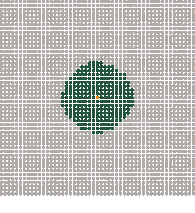
\includegraphics{figures/precompiled/grid_1e-5/points_1.pdf}%
  \quad
  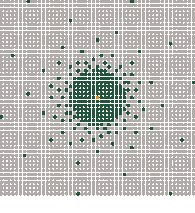
\includegraphics{figures/precompiled/grid_1e-5/points_2.pdf}%
  \quad
  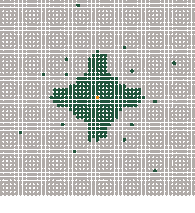
\includegraphics{figures/precompiled/grid_1e-5/points_3.pdf}%
  \quad
  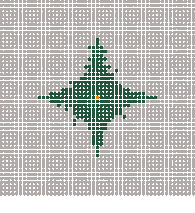
\includegraphics{figures/precompiled/grid_1e-5/points_4.pdf}%
  \caption{
    The first panel shows selecting the \( k \)-\textcolor{seagreen}{nearest
    neighbors} to the \textcolor{orange}{center point} out
    of a dense grid of \textcolor{silver}{candidates}.
    The next panels show selection by greedily maximizing
    conditional mutual information with the center point for a Mat{\'e}rn
    kernel with length scale \( \ell = 1 \) and increasing smoothness \(
    \nu \), from right to left: \( \nu = 1/2, 3/2, 5/2 \).
    The full selections are found at \url{https://youtu.be/lyJf3S5ThjQ}.
  }
  \label{fig:cond_select}
\end{figure}

\section{Sparse Cholesky factorization by KL-minimization}
\label{sec:chol}

Let \( \Theta \in \Reals^{N \times N} \) be a symmetric positive-definite
matrix; we view \( \Theta \) as the covariance matrix of a Gaussian process.
We say that a function \( f(\vec{x}) \) is distributed according to
a Gaussian process prior with mean function \( \mean(\vec{x}) \) and
covariance function or kernel function \( \K(\vec{x}, \vec{x}') \), which
we will denote as \( f(\vec{x}) \sim \GP(\mean(\vec{x}), \K(\vec{x},
\vec{x}')) \), if for any finite set of points \( X = \{ \vec{x}_i \}_{i
= 1}^N \), \( f(X) \sim \N(\vec{\mean}, \CM) \), where \( \mean_i =
\mu(\vec{x}_i) \) and \( \CM_{i, j} = \K(\vec{x}_i, \vec{x}_j) \).

In many applications of Gaussian processes, we
wish to infer unknown data given known data.
Given the training dataset \( \mathcal{D} = \{ (\vec{x}_i, y_i) \}_{i =
1}^N \) where the inputs \( \vec{x}_i \in \Reals^D \) are collected in the
matrix \( X_\Train = [\vec{x}_1, \dotsc, \vec{x}_N]^{\top} \in \Reals^{N
\times D} \) and the measurements at those points are collected in the
vector \( \vec{y}_\Train = [y_1, \dotsc, y_N]^{\top} \in \Reals^N \), we
wish to predict the values at \( m \) new points \( X_\Pred \in \Reals^{m
\times D} \) for which \( \vec{y}_\Pred \in \Reals^m \) is unknown.
We assume the function \( f(\vec{x}) \) that maps input points to their
outputs is distributed according to a Gaussian process with zero mean
function, \( f(\vec{x}) \sim \GP(\vec{0}, \K(\vec{x}, \vec{x}')) \).
From the distribution of \( f(\vec{x}) \), the joint distribution
of training and testing data \( \vec{y} \) has covariance
\(
  \CM =
  \begin{pmatrix}
    \CM_{\Train, \Train} & \CM_{\Train, \Pred} \\
    \CM_{\Pred, \Train} & \CM_{\Pred, \Pred}
  \end{pmatrix}
\)
where \( \CM_{\I, \J} \defeq \K(X_\I, X_\J) \) for index sets \( \I, \J \).
In order to make predictions at \( X_\Pred \), we condition the desired
prediction \( \vec{y}_\Pred \) on the known data \( \vec{y}_\Train \).
For Gaussian processes, the closed-form posterior distribution is
\begin{align}
  \label{eq:cond_mean}
  \E[\vec{y}_\Pred \mid \vec{y}_\Train] &=
    \vec{\mean}_\Pred +
    \CM_{\Pred, \Train} \CM_{\Train, \Train}^{-1}
    (\vec{y}_\Train - \vec{\mean}_\Train) \\
  \label{eq:cond_cov}
  \Cov[\vec{y}_\Pred \mid \vec{y}_\Train] &=
    \CM_{\Pred, \Pred} -
    \CM_{\Pred, \Train} \CM_{\Train, \Train}^{-1}
    \CM_{\Train, \Pred}
 \shortintertext{
    where \( \CM_{\Train, \Train}^{-1} \defeq (\CM_{\Train, \Train})^{-1} \).
    To denote the covariance between the variables in index
    sets \( \I \) and \( \J \), conditional on the variables
    in the index sets \( \V_1, \V_2, \dotsc, \V_n \) we write
  }
  \label{eq:cond_cov_notation}
  \CM_{I, J \mid \V_1, \V_2, \dotsc, \V_n} &\defeq
    \Cov[\vec{y}_\I, \vec{y}_\J \mid
         \vec{y}_{\V_1 \cup \V_2 \cup \dotsb \cup \V_n}].
  \shortintertext{
    We recursively compute \cref{eq:cond_cov_notation}; let \( W = \bigcup_{i
    = 1}^{n - 1} V_i \) and by the quotient rule of Schur complements,
  }
  \label{eq:quotient_rule}
  \CM_{\I, \J \mid \V_1, \dotsc, \V_n} &=
    \CM_{\I,   \J   \mid W} -
    \CM_{\I,   \V_n \mid W}
    \CM_{\V_n, \V_n \mid W}^{-1}
    \CM_{\V_n, \J   \mid W}.
\end{align}

Calculating the posterior mean \cref{eq:cond_mean} and
covariance \cref{eq:cond_cov} requires inverting the training
covariance matrix, usually by means of Cholesky factorization.
The time complexity of computing the Cholesky factorization
is \( \BigO(N^3) \), which is prohibitive for large \( N \).
Thus, we aim to compute \emph{sparse} approximate Cholesky factors.

\subsection{Vecchia approximation}
\label{subsec:vecchia}

The Vecchia approximation for Gaussian processes
\cite{vecchia1988estimation} can be viewed as computing
sparse approximate inverse-Cholesky factors of \( \CM \).
It decomposes the joint likelihood \( \p \) as
\begin{align}
  \label{eq:joint}
  \p(\vec{y}) &= \p(y_1) \p(y_2 \mid y_1) \p(y_3 \mid y_1, y_2) \dotsm
    \p(y_N \mid y_1, y_2, \dotsc, y_{N - 1}).
  \shortintertext{
    The key assumption is that many of the conditioning points are redundant.
    Letting \( i_1, \dotsc, i_N \) denote an ordering of the points and
    \( s_k \) the indices of points that condition the \( k \)th point
    in the ordering, the Vecchia approximation proposes replacing
    \cref{eq:joint} by the sparse approximation
  }
  \label{eq:vecchia}
  \p(\vec{y}) &\approx \p(y_{i_1}) \p(y_{i_2} \mid y_{s_2})
    \p(y_{i_3} \mid y_{s_3}) \dotsm \p(y_{i_N} \mid y_{s_N}).
\end{align}
The precision matrix of the resulting approximate density \cref{eq:vecchia}
has a sparse Cholesky factor in the sense that the \( i \)th column of the
factor has the sparsity pattern \( s_i \) when written in the given elimination
ordering \cite{katzfuss2021general}.
Another way to recover this Cholesky factor for a fixed elimination ordering
\( \prec \) and lower triangular sparsity pattern \( S \defeq \{ (i, j) : i
\in s_j, i \succeq j \} \) is to specify a functional criterion \( \Loss:
\Reals^{N \times N} \to \Reals \) defining an optimization problem over
candidate matrices satisfying the sparsity pattern, \( \SpSet \defeq \{ M
\in \Reals^{N \times N} : M_{i, j} \neq 0 \Rightarrow (i, j) \in S \} \).
\begin{align}
  \label{eq:generic_obj}
  L &\defeq \argmin_{\hat{L} \in \SpSet} \Loss(\hat{L})
\end{align}
Functionals include the Kaporin condition number \( (\trace(L \CM
L^{\top})/N)^N/\det(L \CM L^{\top}) \) \cite{kaporin1990alternative}, the
Frobenius norm \( \norm{\Id - L \chol(\CM)}_{\FRO} \) additionally subject to
the constraint \( \diag(L \CM L^{\top}) = 1 \) \cite{yeremin2000factorized},
and the Kullback-Leiber (KL) divergence \( \KL{\N(\vec{0}, \CM)} {\N(\vec{0},
(L L^{\top})^{-1})} \) \cite{schafer2021sparse}.
These three choices all recover the Vecchia approximation.

As observed in \cite{rue2005gaussian, schafer2021sparse}, factors of the
precision matrix are often much sparser than factors of the covariance
matrix, because the precision encodes conditional independence while the
covariance encodes marginal independence.
The same phenomenon is observed by \cite{spantini2018inference}
working with the more general transport maps.
Covariance matrices arising from kernel functions are often fully
dense, but the approximate factors of their precisions can be
sparse if their ordering and sparsity pattern are chosen carefully.

\subsection{Ordering and sparsity pattern}
\label{subsec:ordering}

Although in this work we primarily focus on constructing
sparsity patterns, the chosen ordering critically affects
the accuracy of lower triangular sparsity patterns.
Vecchia originally proposed ordering points lexicographically, which is
most natural in a one-dimensional setting \cite{vecchia1988estimation}.
More recent work finds that in higher dimensions, exploiting
space-covering orderings leads to significantly better
approximation quality \cite{guinness2018permutation}.
Specifically, we use the maximum-minimum (maximin) ordering
\cite{guinness2018permutation}, which has become popular for the
Vecchia approximation \cite{katzfuss2021general} and Cholesky
factorization \cite{schafer2020compression, schafer2021sparse,
kang2021correlationbased, katzfuss2022scalable}.
The reverse-maximin ordering \( i_1, \dotsc, i_N \) on a set of \( N \) points
\( \{ \vec{x}_i \}_{i = 1}^N \) is defined by first selecting the last index \(
i_N \) arbitrarily and then choosing for \( k = N - 1, N - 2, \dotsc, 1 \) the
index
\begin{align}
  \label{eq:maximin}
  i_k = \argmax_{i \in -\Order_{k + 1}} \; \min_{j \in \Order_{k + 1}}
    \norm{\vec{x}_i - \vec{x}_j}
\end{align}
where \( -\Order \defeq \{ 1, \dotsc, N \} \setminus \Order \)
and \( \Order_n \defeq \{ i_n, i_{n + 1}, \dotsc, i_N \} \),
i.e. select the point farthest from previously selected points.
The ordering is reversed for factorizing the precision.
We write \( i \prec j \) if \( i \) precedes \( j \) in the ordering and
define \( \ell_{i_k} \defeq \min_{j \in \Order_{k + 1}} \norm{\vec{x}_{i_k}
- \vec{x}_j} \), a length scale monotonically shrinking with decreasing
position in the ordering.

Vecchia also originally proposed to select the sparsity set by Euclidean
distance \cite{vecchia1988estimation}, which, unlike the lexicographic
ordering, still remains widely used \cite{schafer2020compression,
schafer2021sparse, katzfuss2022scalable}.
Instead, we will select the sparsity pattern to directly
optimize the accuracy \( \Loss \) \cref{eq:generic_obj}.

\subsection{Review of KL-minimization}
\label{subsec:kl}

The Kullback-Leibler (KL) divergence between two probability distributions \( P
\) and \( Q \) is defined as \( \KL*{P}{Q} \defeq \E_P[\log(\frac{P}{Q})] \).
As the expected difference between true and approximate log-densities, the
KL divergence naturally judges the quality of an approximating distribution.
We identify the positive-definite matrix \( \CM \in \Reals^{N \times N} \)
as the covariance matrix of a centered Gaussian process \( \N(\vec{0}, \CM)
\) which we seek to approximate by a sparse approximate Cholesky factor \(
L \in \SpSet \) of its precision, \( \N(\vec{0}, (L L^{\top})^{-1}) \).
We compare these distributions by the KL divergence as \cite{schafer2021sparse}
does, specializing the generic optimization problem \cref{eq:generic_obj} to
\begin{align}
  \label{eq:L_obj}
  L \defeq \argmin_{\hat{L} \in \SpSet} \,
    \KL*{\N(\vec{0}, \CM)}
        {\N(\vec{0}, (\hat{L} \hat{L}^{\top})^{-1})}.
\end{align}
For multivariate Gaussians, the KL divergence
has a closed-form expression given by
\begin{align}
  \label{eq:kl}
  2 \KL*{\N(\vec{0}, \CM_1)}{\N(\vec{0}, \CM_2)} &=
    \trace(\CM_2^{-1} \CM_1) + \logdet(\CM_2) - \logdet(\CM_1) - N
\end{align}
where \( \CM_1, \CM_2 \in \Reals^{N \times N} \).
Using this expression for the KL divergence and optimizing for \( L \) yields
the following closed-form expression for the nonzero entries in the \( i \)th
column of \( L \) with sparsity pattern \( s_i \), reproduced from Theorem 2.1
of \cite{schafer2021sparse}:
\begin{align}
  \label{eq:L_col}
  L_{s_i, i} &= \frac{\CM_{s_i, s_i}^{-1} \vec{e}_1}
    {\sqrt{\vec{e}_1^{\top} \CM_{s_i, s_i}^{-1} \vec{e}_1}}
\end{align}
where the notation for \( \CM_{s_i, s_i}^{-1} \) is from
\cref{eq:cond_cov_notation} and \( \vec{e}_1 \in \Reals^{\card{s_i}
\times 1} \) denotes the vector with first entry one and the rest zero.
We enforce the convention that \( i \) is the first entry
of \( s_i \), also implying that \( L \) is of full rank.
Plugging the optimal \( L \) \cref{eq:L_col} back into the KL divergence
\cref{eq:kl}, we obtain the objective as a function of the sparsity pattern.
See \cref{app:kl_L} for details; importantly,
the order of the KL divergence matters.
\begin{align}
  \label{eq:obj_chol}
  2 \KL*{\N(\vec{0}, \CM)}{\N(\vec{0}, (L L^{\top})^{-1})} &=
    \sum_{i = 1}^N
      \left [
        \log \left ( \CM_{i, i \mid s_i \setminus \{ i \}} \right ) -
        \log \left ( \CM_{i, i \mid i + 1:} \right )
      \right ]
\end{align}

This sum is the accumulated \emph{difference} in posterior variance for a
series of independent regression problems: each to predict the \( i \)th
variable given a subset of the variables after it in the ordering. The error
\( \log \left ( \CM_{i, i \mid s_i \setminus \{ i \}} \right ) \) made when
restricted to the variables in the sparsity pattern \( s_i \) is compared
to the ground truth \( \log \left ( \CM_{i, i \mid i + 1:} \right ) \).
A similar decomposition of the KL divergence into independent
regression problems was observed in Equation (5) of
\cite{katzfuss2022scalable} for lower triangular transport maps.

Thus, picking the right sparsity pattern to minimize KL divergence reduces
to selecting the points \( s_i \) out of the possible candidates \( i + 1,
\dotsc, N \) that most reduce predictive error at point(s) of interest.
In the next section, we develop such a selection
algorithm for directed inference in Gaussian processes.
We apply this algorithm for sparsity selection of sparse Cholesky factors
in \cref{sec:chol_select} and extend it in \cref{sec:extensions}.

\section{Greedy selection for directed inference}
\label{sec:select}

\begin{figure}[t]
  \centering
  \begin{tikzpicture}[baseline]
  \begin{axis}[
    width={0.4\linewidth},
    axis lines={none},
    scale only axis={true},
    xmin=-1, xmax=1, ymin=-1.5, ymax=1.75,
  ]
  \addplot [only marks, mark size=2, lightblue]
    table {figures/selection/train.csv};
  \addplot [only marks, mark size=4, orange]
    table {figures/selection/test.csv};
  \addplot [only marks, mark size=4, seagreen]
    table {figures/selection/knn_selected.csv};
  \addplot [ultra thick, rust]
    table {figures/selection/knn_mean.csv};
  \addplot [name path=upper, forget plot, draw=none, rust]
    table {figures/selection/knn_std_upper.csv};
  \addplot [name path=lower, forget plot, draw=none, rust]
    table {figures/selection/knn_std_lower.csv};
  \addplot [rust!15] fill between [of=upper and lower];
\end{axis}
\end{tikzpicture}
%
  \begin{tikzpicture}[baseline]
  \begin{axis}[
    width={0.4\linewidth},
    axis lines={none},
    scale only axis={true},
    xmin=-1, xmax=1, ymin=-1.5, ymax=1.75,
  ]
  \addplot [only marks, mark size=2, lightblue]
    table {figures/selection/train.csv};
  \addplot [only marks, mark size=4, orange]
    table {figures/selection/test.csv};
  \addplot [only marks, mark size=4, seagreen]
    table {figures/selection/cknn_selected.csv};
  \addplot [ultra thick, rust]
    table {figures/selection/cknn_mean.csv};
  \addplot [name path=upper, forget plot, draw=none, rust]
    table {figures/selection/cknn_std_upper.csv};
  \addplot [name path=lower, forget plot, draw=none, rust]
    table {figures/selection/cknn_std_lower.csv};
  \addplot [rust!15] fill between [of=upper and lower];
\end{axis}
\end{tikzpicture}

  \caption{
    Here, the \textcolor{lightblue}{blue} points are the
    \textcolor{lightblue}{candidates}, the \textcolor{orange}{orange}
    point is the \textcolor{orange}{target} point to predict
    at, and the \textcolor{seagreen}{green} points are the
    \textcolor{seagreen}{selected} points.
    The \textcolor{rust}{red} line is the \textcolor{rust}{conditional
    mean} \( \mu \), conditional on the selected points, and the \( \pm
    2 \sigma \) \textcolor{rust!60}{confidence interval} is shaded for
    the \textcolor{rust!60}{conditional variance} \( \var \).
    Each method has a budget of two points; the left panel shows selection
    by Euclidean distance and the right by conditional variance.
    Euclidean distance prefers the two points right of the target.
    However, a more balanced view of the situation is obtained when picking
    the slightly farther but
    more informative point to the left,
    reducing variance at the target and thereby reducing predictive error.
  }
  \label{fig:selection}
\end{figure}

In directed Gaussian process regression we are given \( N \) points of
training data and predict at a target point with unknown value by selecting
the \( s \) points most ``informative'' to the target, \(s \ll N \).
From KL-minimization, the criterion for informativity
should be to minimize the variance of the target point,
conditional on the selected points \cref{eq:obj_chol}.
The variance objective was first described by \cite{cohn1996neural} for optimal
experimental design and later applied to directed Gaussian process inference
by \cite{gramacy2014local} who refer to it as the active learning Cohn (ALC)
technique in honor of \cite{cohn1996neural}.
In addition, the variance objective is equivalent to maximizing
the \emph{mutual information} or \emph{information gain} with the
target point as well as minimizing the expected mean squared error
(see \cref{app:mutual_info}).
The mutual information (in a slightly different context) is
also used by \cite{krause2008nearoptimal} for sensor placement.

In contrast to Euclidean distance \cite{vecchia1988estimation} or unconditional
correlation \cite{wada2013gaussian, kang2021correlationbased}, conditional
variance incentivizes the often contradictory demands of being near the target
point (nearby points have higher covariance), but away from previously
selected points (to avoid redundancy); the resulting spread-out selections
are illustrated in \cref{fig:selection}.
Even for isotropic kernels like the Mat{\'e}rn family, the
selections can be anisotropic, as shown in \cref{fig:cond_select}.

\subsection{A greedy approach}
\label{subsec:greedy_select}

Minimizing the conditional variance over all possible \(
\binom{N}{s} \) subsets is intractable, so we greedily select
the next point which most reduces the conditional variance.
Let \( \I = \{ i_j \}_{j = 1}^t \subseteq \Train \) be
the indices of previously selected training points.
For a newly selected index \( k \), we condition the current
covariance matrix on \( y_k \) according to the posterior
\cref{eq:quotient_rule}, resulting in the rank-one downdate
\begin{align}
  \label{eq:cond_select}
  \CM_{:, : \mid \I, k} &= \CM_{:, : \mid \I} - \vec{u} \vec{u}^{\top} &
    \vec{u} &= \frac{\CM_{:, k \mid \I}}{\sqrt{\CM_{k, k \mid \I}}}.
\end{align}
The decrease in the variance of \( y_\Pred \) after
selecting \( k \) is given by \( u_\Pred^2 \), or
\begin{align}
  \label{eq:obj_gp}
  u_\Pred^2
  = \frac{\CM_{\Pred, k \mid \I}^2}{\CM_{k, k \mid \I}}
  = \frac{\Cov[y_\Pred, y_k \mid \I]^2}{\Var[y_k \mid \I]}
  = \Corr[y_\Pred, y_j \mid \I]^2 \Var[y_\Pred \mid \I].
\end{align}
To compute the objective \cref{eq:obj_gp} for each candidate index
\( j \), we start with the unconditional variance \( \CM_{j, j} \)
and covariance \( \CM_{\Pred, j} \), updating these quantities when
an index \( k \) is selected by Equation \cref{eq:cond_select}.
We have two efficient strategies to compute \( \vec{u} \) (as shown in
\cref{fig:alg_update}): either by maintaining the precision of selected
entries \( \CM_{\I, \I}^{-1} \) (\cref{alg:select_prec}) or by storing only
the \( \card{I} \) columns corresponding to selected points from the Cholesky
factor of the joint covariance matrix \( \CM \) (\cref{alg:select_chol});
both methods are detailed in \cref{app:select}.

\begin{figure}[th!]
  \centering
  \begin{minipage}[t]{0.49\textwidth}
    \begin{algorithm}[H]
      \caption{Point selection update \\ by explicit precision}
      \label{alg:update_prec}
      \begin{algorithmic}[1]
  \REQUIRE \(
    X = \begin{pmatrix} X_\Train \\ X_\Pred \end{pmatrix},
    \K(\cdot, \cdot), \I, \CM_{:, : \mid \I}, \CM_{\I, \I}^{-1}, k
  \)
  % \ENSURE \( \I \)

  \STATE \( \I \gets \I \cup \{ k \} \)
  \STATE \( \vec{v} \gets \CM_{\I, \I}^{-1}
    \K(X_{\I \setminus \{ k \}}, X_k) \)
  \STATE \(
    \CM_{\I, \I}^{-1} \gets
    \begin{pmatrix}
      \CM_{\I, \I}^{-1} + \vec{v} \vec{v}^{\top}/\CM_{k, k \mid \I} &
      -\vec{v}/\CM_{k, k \mid \I} \\
      -\vec{v}^{\top}/\CM_{k, k \mid \I} &
      1/\CM_{k, k \mid \I}
    \end{pmatrix}
  \)
  \STATE \( \CM_{:, k} \gets \K(X, X_k) \)
  \STATE \(
    \CM_{:, k \mid \I} \gets \CM_{:, k} -
    \K(X, X_{\I \setminus \{ k \}}) \vec{v}
  \)
  \STATE \(
    \vec{u} \gets \frac{\CM_{:, k \mid \I}}{\sqrt{\CM_{k, k \mid \I}}}
  \)
  \FOR{\( j \in \Train \setminus \I \)}
    \STATE \(
      \CM_{j, j \mid I} \gets
      \CM_{j, j \mid \I} -
      \vec{u}_j^2
    \)
    \STATE \(
      \CM_{j, \Pred \mid \I} \gets
      \CM_{j, \Pred \mid \I} -
      \vec{u}_j \vec{u}_{N + 1}
    \)
  \ENDFOR
\end{algorithmic}

    \end{algorithm}
  \end{minipage}
  \hfill
  \begin{minipage}[t]{0.49\textwidth}
    \begin{algorithm}[H]
      \caption{Point selection update \\ by Cholesky factorization}
      \label{alg:update_chol}
      \begin{algorithmic}[1]
  \REQUIRE \(
    X = \begin{pmatrix} X_\Train \\ X_\Pred \end{pmatrix},
    \K(\cdot, \cdot), \I, \CM_{:, : \mid \I}, L, k
  \)
  % \ENSURE \( \I \)

  \STATE \( \I \gets \I \cup \{ k \} \)
  \STATE \( i \gets \card{\I} \)
  \STATE \( L_{:, i} \gets \K(X, X_k) \)
  \STATE \( L_{:, i} \gets L_{:, i} - L_{:, :i - 1} L_{k, :i - 1}^{\top} \)
  \STATE \( L_{:, i} \gets \frac{L{:, i}}{\sqrt{L_{k, i}}} \)
  \FOR{\( j \in \Train \setminus \I \)}
    \STATE \(
      \CM_{j, j \mid \I} \gets
      \CM_{j, j \mid \I} -
      L_{j, i}^2
    \)
    \STATE \(
      \CM_{j, \Pred \mid \I} \gets
      \CM_{j, \Pred \mid \I} -
      L_{j, i} L_{N + 1, i}
    \)
  \ENDFOR
\end{algorithmic}

    \end{algorithm}
  \end{minipage}
  \caption{Algorithms for updates in single-target selection.}
  \label{fig:alg_update}
\end{figure}

Both approaches have a time complexity of \( \BigO(N s^2) \) to select
\( s \) points out of \( N \) candidates, differing in space complexity.
The precision takes \( \BigO(s^2) \) space while the first
\( s \) columns of the Cholesky factor of \( \CM \) uses
\( \BigO(N s) \) space, always more memory (\( N > s \)).
Both algorithms use \( \BigO(N) \) space
to store the conditional (co)variances.
The precision algorithm uses less memory than the Cholesky algorithm.
However, the Cholesky algorithm is easier to implement and
roughly two times faster, which is why we use it in practice.

\section{Greedy selection for global approximation by KL-minimization}
\label{sec:chol_select}

\begin{figure}[t]
  \centering
  % left matrix
\fill[lightsilver,opacity=0.5]   (0,        0) rectangle (1, -1);
\fill[lightblue,  opacity=0.5]   (0,    -0.75) rectangle (0.75, -1);
\fill[lightblue,  opacity=0.5]   (0.75,     0) rectangle (1, -0.75);
\fill[lightblue,  opacity=1.0]   (0.75, -0.75) rectangle (1, -1);

% equals sign
\node at (1.25, -0.5) {\Huge \textcolor{darksilver}{$=$}};

% lower triangle
\fill[lightsilver,opacity=0.5]
(1.5, -1) -- (2.5, -1) -- (1.5, 0) -- cycle;
\fill[lightblue,  opacity=1.0]
(1.5, -1) -- (2.5, -1) -- (2.25, -0.75) -- (1.5, -0.75) -- cycle;

% times
\node at (2.05, -0.5) {\Huge \textcolor{darksilver}{$\cdot$}};

% upper triangle
\fill[lightsilver,opacity=0.5]
(2.6, -1) -- (2.6, 0) -- (1.6, 0) -- cycle;
\fill[lightblue,  opacity=1.0]
(2.6, -1) -- (2.6, 0) -- (2.35, 0) -- (2.35, -0.75) -- cycle;

%
  \qquad
  \begin{tikzpicture}[baseline]
  \begin{axis}[
    % calculated from Cholesky factor, exactly 16 cm x 16 cm
    width={4cm},
    height={4cm},
    axis lines={none},
    % force axis box to have exactly the right dimensions, ignoring labels
    scale only axis=true,
  ]
  % consistent size bounding box
  \draw [white, line width=0] (-0.1, -0.1) -- (-0.1,  1.1);
  \draw [white, line width=0] ( 1.1, -0.1) -- ( 1.1,  1.1);
  \draw [white, line width=0] (-0.1, -0.1) -- (-1.1, -0.1);
  \draw [white, line width=0] (-0.1,  1.1) -- (-1.1,  1.1);
  % \addplot [only marks, mark size=1, silver]    table
  %  {figures/points/all_points.csv};
  \addplot [only marks, mark size=2, lightblue] table
    {figures/points/candidates.csv};
  \addplot [only marks, mark size=4, seagreen]  table
    {figures/points/selected.csv};
  \addplot [only marks, mark size=4, orange]    table
    {figures/points/target.csv};
  \end{axis}
\end{tikzpicture}

  \caption{
    For a column of a Cholesky factor in isolation, the
    \textcolor{orange}{target} point is the \textcolor{orange}{diagonal}
    entry, \textcolor{lightblue}{candidates} are \textcolor{lightblue}{below}
    it, and the \textcolor{seagreen}{selected} entries are added to
    the \textcolor{seagreen}{sparsity pattern}.
    Points violating lower triangularity are
    not shown.
    Thus, sparsity selection in Cholesky factorization
    (left panel) is analogous to training point selection
    in directed Gaussian process regression (right panel).
  }
  \label{fig:select_chol}
\end{figure}

Directed Gaussian process regression infers the
\emph{local} distribution at points of interest.
We now turn our attention to \emph{global} approximation of the entire Gaussian
process; given a kernel function \( \K(\vec{x}, \vec{x}') \) and a set of \(
N \) points \( \{ \vec{x}_i \}_{i = 1}^N \) we have the covariance matrix \(
\CM_{ij} = K(\vec{x}_i, \vec{x}_j) \) for which we seek a sparse approximate
Cholesky factor \( L \) of the precision, \( L L^{\top} \approx \CM^{-1} \).
We first order the points by the reverse-maximin ordering described in
\cref{subsec:ordering} and then apply the selection
algorithm developed in \cref{sec:select} to form the sparsity pattern.
For the \( i \)th column of \( L \), the target point is the \( i \)th point
in the ordering, the candidate points are those satisfying lower triangularity
(after the target in the ordering), and running the selection algorithm for
the desired number of nonzeros entries picks out indices which we add to the
sparsity set \( s_i \); this process is illustrated in \cref{fig:select_chol}.
Finally, we compute the values of the selected nonzero
indices by the closed-form expression \cref{eq:L_col}.
Both sparsity selection and computing entries are
embarrassingly parallel over \( L \)'s columns.

Using the single-target algorithm from \cref{subsec:greedy_select}
has time complexity \( \BigO(N C s^2) \) to select \( s \)
nonzero entries out of \( C \) candidates for \( N \) columns.
Computing the corresponding values \( \CM_{s_i, s_i}^{-1}
\vec{e}_1 \) has time complexity \( \BigO(N s^3) \).
Sparsity selection has the same complexity as entry computation
if the number of candidates \( C \) is \( \BigO(s) \), suggesting
the need to limit the number of candidates considered.
In practice, we pick the candidate set to be the nearest neighbors
of the point of interest as \cite{gramacy2014local} does;
specifically, we use the framework of \cite{schafer2021sparse}
which considers all points within a radius proportional to the
length scale from the reverse-maximin ordering \cref{eq:maximin}.

\section{Extensions}
\label{sec:extensions}

Here we consider extensions of the basic single-column
method to aggregated (or supernodal) Cholesky factorization
and to determining the number of nonzeros per column.
Numerical experiments are presented in \cref{sec:experiments}.

\subsection{Aggregated sparsity pattern}
\label{subsec:aggregated}

We now derive a similar decomposition of the KL divergence
if the same sparsity pattern is reused for multiple columns,
known as aggregated or supernodal Cholesky factorization.
Aggregation can lead to substantial time
and space savings \cite{schafer2021sparse}.
For this section we focus on a single group \( \tilde{i}
= \{i_1, \dotsc, i_m \} \) obtained by aggregating the
column indices \( i_1 \succ i_2 \succ \dotsb \succ i_m \).
Let \( \tilde{i} \) have aggregated selected entries \(
s_{\tilde{i}} \) satisfying \( s_{\tilde{i}} \supseteq \tilde{i}
\) to guarantee that the Cholesky factor has full rank.
Let \( \tilde{s} \defeq s_{\tilde{i}} \setminus \tilde{i} \)
be the selected entries excluding the columns in the group.
The sparsity pattern for the \( k \)th column in the group is then the
aggregated selected entries excluding the entries that violate lower
triangularity, \( s_k \defeq \{ j \in s_{\tilde{i}} : j \succeq k \} \).
Assuming every entry of \( \tilde{s} \) is after every index in \( \tilde{i}
\), then \( s_k = \tilde{s} \cup \{ j \in \tilde{i} : j \succeq k \} \).
This condition is guaranteed if the aggregated columns are adjacent in the
ordering, for example; we defer handling the general case to the next section.
The KL divergence \cref{eq:obj_chol} restricted to
the contribution from the group \( \tilde{i} \) is
\begin{align}
  \label{eq:obj_mult}
  \sum_{i \in \tilde{i}}
    \log \left (\CM_{i, i \mid s_i \setminus \{ i \} } \right ) &=
    \logdet(\CM_{\tilde{i}, \tilde{i} \mid \tilde{s}})
\end{align}
from \cref{app:kl_agg}.
Thus, the generalization of the posterior variance
\cref{eq:obj_chol} to aggregated columns is their log
determinant conditional on (well-behaved) selected entries.
We briefly discuss what happens when
selected entries are \emph{between} columns.

\subsubsection{Nonadjacent or partial aggregation}
\label{subsubsec:partial}

Let the random variables corresponding to the indices \( \tilde{i} = \{
i_1, \dotsc, i_m \} \) be collected in a vector \( \vec{y} = [y_1, \dotsc,
y_m]^{\top} \) with joint density \( \vec{y} \sim \N(\vec{0}, \CM) \).
We select a random variable with index \( k \) and define \emph{partial}
conditioning to mean that \( k \) conditions all but the first \( p \)
variables (recall that the indices are sorted w.r.t \( \succ \), so if
\( k \) conditions a variable, it conditions all those afterwards).
We denote the partial conditioning of \( y \) as \( \vec{y}_{\parallel
k} \defeq [y_1, \dotsc, y_p, y_{p + 1 \mid k}, \dotsc, y_{m \mid k}]^{\top}
\) and its covariance matrix \( \Cov[\vec{y}_{\parallel k}] \) as
\begin{align}
  \label{eq:chol_partial}
  \CM_{\tilde{i}, \tilde{i} \parallel k} &\defeq
  \Cov[\vec{y}_{\parallel k}] =
  \begin{pmatrix}
    L_{:p} L_{:p}^{\top} &
    L_{:p} {L'}_{p + 1:}^{\top} \\
    {L'}_{p + 1:} L_{:p}^{\top} &
    {L'}_{p + 1:} {L'}_{p + 1:}^{\top}
  \end{pmatrix} =
  \begin{pmatrix}
    L_{:p} \\
    {L'}_{p + 1:}
  \end{pmatrix}
  \begin{pmatrix}
    L_{:p} \\
    {L'}_{p + 1:}
  \end{pmatrix}^{\top}
\end{align}
where \( L = \chol(\CM) \) and \( L' = \chol(\CM_{:, : \mid k}) \).
See \cref{fig:partial_factor} for an
illustration and \cref{app:partial} for details.
Armed with this representation, we compute \(
\logdet(\CM_{\tilde{i}, \tilde{i} \parallel k}) \):
\begin{align}
  \label{eq:partial_kl}
  \sum_{i \in \tilde{i}}
    \log \left (\CM_{i, i \mid s_i \setminus \{ i \} } \right ) &=
    \logdet(\CM_{\tilde{i}, \tilde{i} \parallel k}).
\end{align}
Like the aggregated case \cref{eq:obj_mult}, minimizing the log determinant
of the \emph{partially} conditioned covariance matrix \cref{eq:chol_partial}
is the same as minimizing the KL divergence \cref{eq:obj_chol}.

\subsection{Supernodes and blocked selection}
\label{subsec:mult_select}

For multiple (\( m > 1 \)) target points, \cite{gramacy2014local} suggests
independently applying the single-target algorithm to each target.
Instead, we will use \emph{the same} selected points for \emph{all} the
target points, essentially speeding up selection by a factor of \( m \).
Furthermore, the cost of computing the entries of the
resulting Cholesky factor is reduced by this aggregation.
The primary downside is reduced accuracy per sparsity entry
since each target no longer receives individual attention.
We mitigate this by paying heed to the ``two birds with
one stone'' maxim, or by considering a candidate's
simultaneous effect on \emph{all} prediction points.
In practice, this approach yields better accuracy
per unit time than single-target selection.

The first question is how to generalize the objective for
a single target \cref{eq:obj_gp} to multiple targets.
Continuing with KL-minimization \cref{eq:obj_mult}, the criterion
should be to minimize the log determinant of the posterior
covariance matrix, \( \logdet(\CM_{\Pred, \Pred \mid I}) \).
This objective, known as D-optimal design in the literature
\cite{krause2008nearoptimal}, can be intuitively interpreted as a volume of
uncertainty or as a scaling factor in the density of multivariate Gaussians.
In addition, it is equivalent to maximizing mutual information
since the differential entropy of a Gaussian strictly increases
with its log determinant (see \cref{app:mutual_info}).

We want to quickly compute how selecting an
index \( k \) affects the log determinant.
By application of the matrix determinant lemma
(the details are in \cref{app:logdet_downdate}),
\begin{align}
  \label{eq:greedy_mult}
  \logdet(\CM_{\Pred, \Pred \mid \I, k})  - \logdet(\CM_{\Pred, \Pred \mid \I})
  &= \log(\CM_{    k,     k \mid \I, \Pred}) - \log(\CM_{    k,     k \mid \I}).
\end{align}
Equation \cref{eq:greedy_mult} swaps the roles of the targets
and the candidate: the \emph{candidate} is now conditioned
by the \emph{targets}, reducing to single-target selection.
Using the recipes from \cref{subsec:greedy_select} to compute conditional
variances, we can compute the objective by maintaining a data structure
for each term: one for \( \CM_{k, k \mid \I, \Pred} \) and the other for
\( \CM_{k, k \mid \I} \).
By the quotient rule \( \CM_{k, k \mid \I, \Pred} = \CM_{k,
k \mid \Pred, \I} \), so we can condition on the prediction
points \emph{before} any points have been selected.
After this initialization, we repeatedly update both data structures after
selecting the best candidate by the objective \cref{eq:greedy_mult}.

We have two strategies from the two approaches of the single-target
algorithm: one maintaining the precision of the selected entries \( \CM_{\I,
\I}^{-1} \) as well as of the target points \( \CM_{\Pred, \Pred}^{-1} \)
(\cref{alg:select_mult_prec}) and the other simply storing two Cholesky factors
of the joint covariance matrix \( \CM \) (\cref{alg:select_mult_chol}); both
methods are detailed in \cref{app:mult_select}.

Both approaches have a time complexity of \( \BigO(N s^2 + N m^2 + m^3) \) to
select \( s \) points out of \( N \) candidates for \( m \) targets, again
differing in space complexity: although using more memory, the Cholesky
approach is preferred for simplicity and performance.

\paragraph{Partial selection}

The multiple-target algorithm implicitly assumes that a candidate
conditions \emph{every} target point. 
However, candidates
can also condition only a subset of the targets in the aggregated
Cholesky factorization setting of \cref{subsubsec:partial}.
Proper ``partial'' selection accounting for this structure is able to match
the asymptotic time and space complexities of the multiple-target algorithm
by also storing a partial Cholesky factor, the details are provided in
\cref{subsec:partial_select} and \cref{alg:select_partial}.

\subsection{Aggregated Cholesky}

In an aggregated sparsity pattern, columns are partitioned into groups and
selecting an index for a group \( \tilde{i} \) adds it to the sparsity.

We group columns by the framework of \cite{schafer2021sparse} which aggregates
points that are close both geometrically as well as in the ordering.
To select sparsity entries, the targets are all points in \( \tilde{i} \)
and the candidates are the union of the nearest neighbors to each target.
If every candidate \( k \) satisfies \( k \succ \max{\tilde{i}} \) which
occurs if the group is contiguous in the ordering e.g., then every candidate
conditions every target and so the multiple-target selection algorithm
(\cref{subsec:mult_select}) can be directly applied.
However, we empirically observe that forcing this condition irreparably
damages the accuracy of the resulting factor: forming groups contiguous in
the ordering no longer guarantees that grouped points are spatially close,
and removing candidates between targets filters many of them out.
If the condition is not forced, then selecting candidates can
condition subsets of the group; the multiple-target algorithm
now systematically overestimates the effect on targets.
Using the partial selection algorithm (\cref{subsec:partial_select})
instead on unmodified grouping and candidate sets
significantly improves the approximation quality.

Because the sparsity patterns for columns in the same group are subsets
of each other, we can efficiently compute the group's entries in \( L \)
\cref{eq:L_col} together in the time complexity for a single column (see
\cref{app:L_mult} or Algorithm 3.2 of \cite{schafer2021sparse}).
If each group has \( m \) points, both the multiple-target and
partial algorithms have time complexity \( \BigO(C s^2 + C m^2
+ m^3) \) to select \( s \) points out of \( C \) candidates.
Over \( N/m \) groups the time complexity for both selection and entry
computation is \( \BigO(\frac{N}{m} (C s^2 + C m^2 + m^3 + s^3)) \),
simplifying to \( \BigO(\frac{N C s^2}{m}) \) assuming \( m = \BigO(s) \),
a \( m \) times improvement over non-aggregated factorization.
Better time complexity yields denser and thereby
more accurate factors in the same amount of time.
However, the sparsity pattern is no longer tailored to particular columns
since it is shared within a group.
This means the aggregated factor is less efficient
at reducing the KL divergence per nonzero.

\subsection{Allocating nonzeros by global greedy selection}
\label{subsec:global_greedy}

Given a budget on the total number of nonzeros, one
must decide how many nonzeros to assign to each column.
We recommend the simple strategy of distributing nonzeros as evenly as
possible, maximizing computational efficiency since denser columns have
an outsized impact on the computational time from the cubic scaling cost
with the number of nonzeros.

In inhomogeneous geometries where certain points benefit from
more nonzeros than others, a principled way of distributing nonzeros is to
minimize KL divergence end-to-end like was done for sparsity selection.
The \emph{local} greedy algorithms select the sparsity entry that
minimizes prediction error at \emph{particular} columns of interest.
In \emph{global} greedy selection, we pick from \emph{any} column the
candidate that minimizes the overall KL divergence \cref{eq:obj_chol}.
We maintain a priority queue containing all candidates from every
column, keyed by the candidate's effect on the KL divergence.
The data structure must support popping the largest element off the
queue as well as updating the value for an element in the queue.
Both operations have time complexity \( \BigO(\log n) \) for \( n \)
elements if implemented as an array-backed binary heap, for example.

The greedy selection algorithms already compute the effect of
an entry on the KL divergence, up to monotonically increasing
transformations (which preserve the ranking of candidates).
But in the global context, if different columns use different
transformations, then the ranking of candidates between columns is skewed.
We describe the necessary modifications to
compute exactly the difference in KL divergence.

\subsubsection{Single column selection}
\label{subsubsec:single_column}

Selecting an entry \( k \) for a single target only affects its conditional
variance, so exactly one term in the KL divergence \cref{eq:obj_chol} changes,
\begin{align}
  \argmin_k \left [
    \log(\CM_{\Pred, \Pred \mid \I, k}) - \log(\CM_{\Pred, \Pred \mid \I})
  \right ] &=
    \argmin_k \left (
      \CM_{\Pred, \Pred \mid \I, k}
    \right ) \CM_{\Pred, \Pred \mid \I}^{-1}.
  \shortintertext{
    Using the original objective \cref{eq:obj_gp} to
    compute the change in variance from selecting \( k \),
  }
  \label{eq:global_obj}
  \argmin_k \left (
    \CM_{\Pred, \Pred \mid \I} -
      \frac{\CM_{\Pred, k \mid \I}^2}{\CM_{k, k \mid \I}}
  \right ) \CM_{\Pred, \Pred \mid \I}^{-1} &=
    \argmax_k \; \Corr[y_\Pred, y_k \mid \I]^2
\end{align}
where the new objective \cref{eq:global_obj} is easily computed as
the original objective \cref{eq:obj_gp} divided by the target's
conditional variance, the percentage the decrease in variance takes up.

\subsubsection{Aggregated selection}
\label{subsubsec:mult_column}

The multiple-target algorithm already computes the exact
difference in log determinant after selecting a candidate.
The partial selection algorithm computes the log determinant itself, not
the difference, so the log determinant before the selection needs to be
subtracted, easily computed as the sum of the squared ``diagonal'' entries
of \( L \) corresponding to target points from \cref{eq:partial_diag}.

% One heuristical improvement is to measure ``bang for the buck'',
% i.e. to consider that the number of nonzeros added from selecting
% a candidate varies depending on the number of targets conditioned.
% The KL divergence adds a candidate's effect on each target together,
% so candidates conditioning more targets tend to decrease the KL
% divergence more, even if they are less efficient per target.
% In practice, it is often better to divide the change
% in KL divergence by the number of targets conditioned.
%
% For the multiple-target algorithm, this modification makes no difference
% within a group since every candidate conditions every target point, but can
% make a difference in the global setting if groups have different sizes.
% This modification can make a difference both within a column and
% globally for the partial algorithm since different candidates
% within the same group can condition a different number of targets.

\section{Numerical experiments}
\label{sec:experiments}

All experiments ran on the Partnership for an Advanced Computing Environment
(PACE) Phoenix cluster at the Georgia Institute of Technology, with 8
cores of a Intel Xeon Gold 6226 CPU @ 2.70GHz and 22 GB of RAM per core.
The code is written in Python using standard scientific libraries
\texttt{numpy} \cite{harris2020array}, \texttt{scipy} \cite{virtanen2020scipy},
\texttt{scikit-learn} \cite{pedregosa2011scikitlearn}, \texttt{matplotlib}
\cite{hunter2007matplotlib} as well as Cython \cite{behnel2011cython} which
provides direct transpilation of Python code into C.
Cython also allows Python code to access native C interfaces
to the \texttt{BLAS} and Intel \texttt{oneMKL} libraries.
Code for all numerical experiments can be found at
\href{https://github.com/stephen-huan/conditional-knn}
{https://github.com/stephen-huan/conditional-knn}.

\subsection{Cholesky factorization}
\label{subsec:chol_exp}

We empirically verify that conditional sparsity selection
produces more accurate sparse Cholesky factors than
selection by Euclidean distance at the same density.
We take \( N \) points on a slightly perturbed regular
grid in \( [0, 1]^2 \) and use a Mat{\'e}rn kernel with
smoothness \( \nu = 5/2 \) and length scale \( \ell = 1 \).

As a baseline for comparison, we use the single-column and aggregated variants
of the KL-minimization framework of \cite{schafer2021sparse}, which orders
points by the reverse-maximin ordering described in \cref{subsec:ordering} and
forms the sparsity pattern by selecting all points within a radius of \( \rho
\ell_i \) to the \( i \)th point, where \( \rho \geq 1 \) is a tuning parameter
for density and \( \ell_i \) is the length scale from the reverse-maximin
ordering.
We also try selecting points by \( k \)-nearest neighbors (\( k \)-NN),
where \( k \) is chosen to match the number of nonzeros of the baseline.

For our method, we run the baseline with a larger \( \rho' = \rho_s
\cdot \rho \) to get an initial candidate set where \( \rho_s \)
is a tuning parameter for the number of candidates considered.
If not stated otherwise, \( \rho_s = 2 \) is used in the following experiments.
We then use the single-column and partial variants of the conditional
selection algorithm described in \cref{sec:select} to subsample the
actual sparsity entries from the candidate set; in these experiments,
each column receives \( k \) nonzeros where \( k \) is chosen to match
the original density \( \rho \) of the baseline factor.
In this setting we found that using the global
selection procedure described in \cref{subsec:global_greedy} to
determine the number of nonzeros for each column led to little
improvement in accuracy at a significant performance penalty.

We aggregate columns by the procedure of \cite{schafer2021sparse}: pick
the first (w.r.t \( \prec \)) index \( i \) that has not been aggregated
and create the group \( \{ j: j \in s_i, \ell_j \leq \lambda \ell_i \} \)
where \( \lambda \geq 1 \) is a tuning parameter for group size; repeat
until all indices have been aggregated.
We generate the groups using the sparsity pattern
from the baseline factor and use the same groups for
aggregated conditional selection for a fair comparison.
In all experiments we use \(\lambda = 1.5 \)
as recommended by \cite{schafer2021sparse}.

As \cref{fig:chol_n} shows, the KL divergence and computational
time increase linearly with the number of points for all methods.
Conditional methods are more accurate than their unconditional
counterparts and the denser aggregated variants are both more
accurate and faster than their non-aggregated counterparts.

\cref{fig:chol_rho} shows that the conditional selection methods achieve
significantly better KL divergence compared to their unconditional
counterparts for the same number of entries of the sparsity set.
However, they do not achieve better accuracy per
unit time cost from the increased cost of selection.
Aggregation results in better accuracy per unit time cost but worse accuracy
per nonzero entry, which may impact their computational efficiency in
downstream tasks which depend on factor density like preconditioning.

\pgfplotsset{
  cycle list={
    {very thick, lightblue, style=dashed,         mark=*},
    {very thick, seagreen,  style=dashdotted,     mark=o},
    {very thick, silver,    style=densely dotted, mark=triangle*},
    {very thick, orange,    style=solid,          mark=square*},
    {very thick, rust,      style=dotted,         mark=square},
  }
}

\begin{figure}[t]
  \centering
  \begin{tikzpicture}[baseline, scale=0.75]
  \begin{axis}[
    grid={major},
    % title={KL divergence with increasing \( N \)
    %   (\( \rho = 2, \rho_s = 2, \lambda = 1.5 \))},
    xlabel={\( N \)},
    ylabel={KL divergence},
    legend entries={KL, KL (agg.), select (\( k \)-NN), select, select (agg.)},
    legend pos={north west},
  ]
  \addplot [very thick, lightblue]  table
    {figures/cholesky/n_kl_div_KL.csv};
  \addplot [very thick, seagreen]   table
    {figures/cholesky/n_kl_div_KL_agg.csv};
  \addplot [very thick, darksilver] table
    {figures/cholesky/n_kl_div_select-KNN.csv};
  \addplot [very thick, orange]     table
    {figures/cholesky/n_kl_div_select.csv};
  \addplot [very thick, rust]       table
    {figures/cholesky/n_kl_div_select_agg.csv};
  \end{axis}
\end{tikzpicture}
%
  \begin{tikzpicture}
  \begin{axis}[
    width={0.8\linewidth},
    grid={major},
    % title={Time with increasing \( N \)
    % (\( \rho = 2, \rho_s = 2, \lambda = 1.5 \))},
    xlabel={\( N \)},
    ylabel={Time (seconds)},
    legend entries={kl, kl (agg), select (knn), select, select (agg)},
    legend pos={north west},
  ]
  \addplot [lightblue]  table {figures/cholesky/n_time_KL.csv};
  \addplot [seagreen]   table {figures/cholesky/n_time_KL_agg.csv};
  \addplot [darksilver] table {figures/cholesky/n_time_select-KNN.csv};
  \addplot [orange]     table {figures/cholesky/n_time_select.csv};
  \addplot [rust]       table {figures/cholesky/n_time_select_agg.csv};
  \end{axis}
\end{tikzpicture}

  \caption{
    Accuracy (left) and computational time (right) of
    Cholesky factorization methods with varying number
    of points \( N \) and fixed density \( \rho = 2 \).
    ``KL'' is the baseline from \cite{schafer2021sparse}, ``\( k
    \)-NN'' is selection by \( k \)-nearest neighbors, ``select''
    is conditional selection, and ``(agg.)'' denotes aggregation.
  }
  \label{fig:chol_n}
\end{figure}

\begin{figure}[t]
  \centering
  \begin{tikzpicture}[baseline, scale=0.75]
  \begin{semilogyaxis}[
    grid={major},
    % title={KL divergence with increasing nonzeros
    %   (\( N = 65536, \rho_s = 2, \lambda = 1.5 \))},
    xlabel={Nonzeros (nnz)},
    ylabel={\( \log_{10} \) KL divergence},
    legend entries={%
      \( \rho \)-ball, \( \rho \)-ball (agg.),
      \( k \)-NN, select, select (agg.)
    },
    legend pos={north east},
  ]
  \addplot table {figures/cholesky/rho_kl_div_KL.csv};
  \addplot table {figures/cholesky/rho_kl_div_KL_agg.csv};
  \addplot table {figures/cholesky/rho_kl_div_select-KNN.csv};
  \addplot table {figures/cholesky/rho_kl_div_select.csv};
  \addplot table {figures/cholesky/rho_kl_div_select_agg.csv};
  \end{semilogyaxis}
\end{tikzpicture}
%
  \begin{tikzpicture}[baseline, scale=0.75]
  \begin{loglogaxis}[
    grid={major},
    % title={KL divergence against time with increasing \( \rho \)
    %   (\( N = 65536, \rho_s = 2, \lambda = 1.5 \))},
    xlabel={\( \log_{10} \) Time (seconds)},
    % legend entries={KL, KL (agg.), select (\( k \)-NN), select, select (agg.)},
    % legend pos={north east},
  ]
  \addplot table {figures/cholesky/rho_time_KL_kl_div.csv};
  \addplot table {figures/cholesky/rho_time_KL_agg_kl_div.csv};
  \addplot table {figures/cholesky/rho_time_select-KNN_kl_div.csv};
  \addplot table {figures/cholesky/rho_time_select_kl_div.csv};
  \addplot table {figures/cholesky/rho_time_select_agg_kl_div.csv};
  \end{loglogaxis}
\end{tikzpicture}

  \caption{
    The left panel shows the KL divergence with varying
    density \( \rho \) and the right panel shows the accuracy
    to computational time trade-off over varying \( \rho \).
    The number of points is \( N = 2^{16} \).
  }
  \label{fig:chol_rho}
\end{figure}

\subsection{Gaussian process regression}
\label{subsec:gp_exp}

For Gaussian process regression we use the ``predictions points first''
method of \cite{schafer2021sparse} which computes a sparse Cholesky factor
of the joint covariance matrix between the training and prediction points,
where prediction points are ordered before training points.
The desired posterior mean and covariance can then be
computed efficiently from sparse submatrices of the factor.
See subsection 4.2.1, Appendix D.1, or Algorithm D.1
of \cite{schafer2021sparse} for additional details.

\begin{figure}[t]
  \centering
  % \begin{tikzpicture}[baseline]
  \begin{axis}[
    width={\linewidth},
    height={0.5\linewidth},
    ticks=none,
  ]
  \addplot [only marks, mark size=0.6, silver] table
    {figures/datasets/sarcos/sarcos.csv};
  \end{axis}
\end{tikzpicture}

  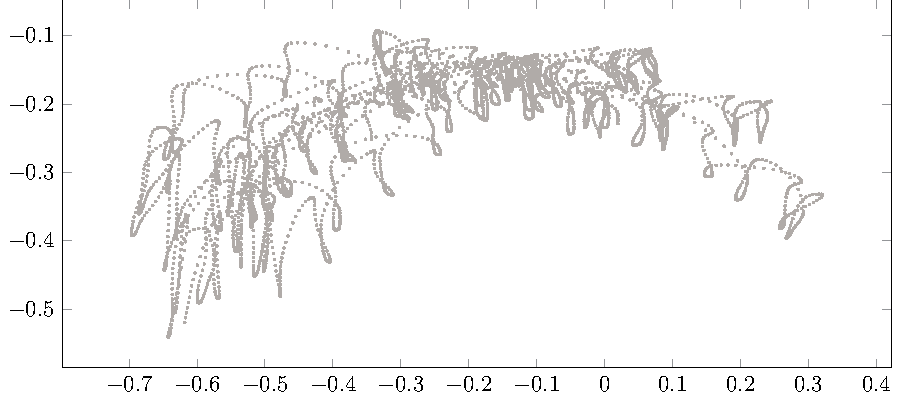
\includegraphics{figures/precompiled/datasets/sarcos.pdf}
  \caption{
    The first 5,000 points of the SARCOS training
    data, visualizing the first two features.
  }
  \label{fig:sarcos}
\end{figure}

\subsubsection{SARCOS dataset}

We use the SARCOS dataset \cite{vijayakumar2000locally} generated from
an inverse dynamics problem on a 7 degrees-of-freedom robotic arm.
Given 7 joint positions, velocities, and accelerations for 21 features
in total, the goal is to infer the torque of just the first joint.
The dataset is available online at \url{https://gaussianprocess.org/gpml/data/}
and consists of 44,484 training points and 4,449
testing points which we then preprocess as follows.

We only use the first 3 features of the data and
remove the 73 duplicate points this projection causes.
Since the provided testing points overlap significantly with the training
points, we ignore the original testing points and instead randomly partition
the 44,411 remaining training points into 90\% training points (\( N = 39,969
\)) and 10\% prediction points (\( m = 4,442 \)).
Since the robot arm moves smoothly, the geometry of the dataset consists
of relatively continuous overlapping paths as shown in \cref{fig:sarcos}.
We then use a Mat{\'e}rn kernel with smoothness \( \nu = 3/2 \) and length
scale \( \ell = 1 \) and draw \( 10^3 \) realizations from the resulting
Gaussian process for the target variable, ignoring the original objective
to ensure that the target variable is exactly Gaussian.

We consider three accuracy metrics for Gaussian process regression:
the log determinant of the posterior prediction covariance matrix,
the empirical coverage of the 90\% posterior prediction intervals
averaged over all realizations, and the average root mean square
error (RMSE) of the posterior means.
The log determinant is equivalent to the KL divergence by the
discussion in \cref{subsec:aggregated}, so the results are
similar to Cholesky factorization (\cref{subsec:chol_exp}).
We find that coverage is extremely accurate for all
methods (within \( 0.1\% \) for \( \rho > 2 \)).
Finally, the RMSE is shown in \cref{fig:gp_sarcos_rho}.

Despite an increased cost to select points, the conditional methods have
better accuracy per unit computational cost than their unconditional
counterparts as a result of their superior accuracy at the same sparsity.
However, the simpler method of \( k \)-NN also
achieves comparable accuracy per unit time cost.
As noted in \cite{gramacy2015speeding}, the simple method of
\( k \)-NN remains hard to beat without specialized tricks.

\begin{figure}[t]
  \centering
  \begin{tikzpicture}[baseline, scale=0.75]
  \begin{loglogaxis}[
    grid={major},
    % title={RMSE with increasing \( \rho \)
    %   (\( N = 44411, \rho_s = 2, \lambda = 1.5 \))},
    xlabel={\( \log_{10} \) Nonzeros (nnz)},
    ylabel={\( \log_{10} \) RMSE},
    % legend entries={KL, KL (agg.), \( k \)-NN, select, select (agg.)},
    % legend pos={north east},
  ]
  \addplot table {figures/gp/sarcos/rho_loss_KL.csv};
  \addplot table {figures/gp/sarcos/rho_loss_KL_agg.csv};
  \addplot table {figures/gp/sarcos/rho_loss_select-KNN.csv};
  \addplot table {figures/gp/sarcos/rho_loss_select.csv};
  \addplot table {figures/gp/sarcos/rho_loss_select_agg.csv};
  \end{loglogaxis}
\end{tikzpicture}
%
  \begin{tikzpicture}[baseline, scale=0.75]
  \begin{loglogaxis}[
    grid={major},
    % title={RMSE against time with increasing \( \rho \)
    %   (\( N = 44411, \rho_s = 2, \lambda = 1.5 \))},
    xlabel={\( \log_{10} \) Time (seconds)},
    % ylabel={\( \log_{10} \) RMSE},
    legend entries={KL, KL (agg.), \( k \)-NN, select, select (agg.)},
    legend pos={north east},
    legend style={nodes={scale=0.9, transform shape}},
  ]
  \addplot table {figures/gp/sarcos/rho_time_KL_loss.csv};
  \addplot table {figures/gp/sarcos/rho_time_KL_agg_loss.csv};
  \addplot table {figures/gp/sarcos/rho_time_select-KNN_loss.csv};
  \addplot table {figures/gp/sarcos/rho_time_select_loss.csv};
  \addplot table {figures/gp/sarcos/rho_time_select_agg_loss.csv};
  \end{loglogaxis}
\end{tikzpicture}

  \caption{
    We perform Gaussian process regression by sparse
    Cholesky factorization of the joint covariance matrix.
    Like Cholesky factorization in \cref{subsec:chol_exp}, we
    use a candidate set size scaling factor of \( \rho_s = 2
    \) and an aggregation parameter of \( \lambda = 1.5 \).
    The left panel shows the difference in RMSE from exact Gaussian process
    regression using the same training points with varying density \( \rho \).
    The right panel shows the accuracy to computational
    time trade-off over varying \( \rho \).
  }
  \label{fig:gp_sarcos_rho}
\end{figure}

\begin{figure}[t]
  \centering
  % \begin{tikzpicture}[baseline]
  \begin{axis}[
    width={\linewidth},
    height={0.5\linewidth},
    % ticks=none,
  ]
  \addplot [only marks, mark size=0.6, silver] table
    {figures/datasets/oco2/oco2.csv};
  \end{axis}
\end{tikzpicture}

  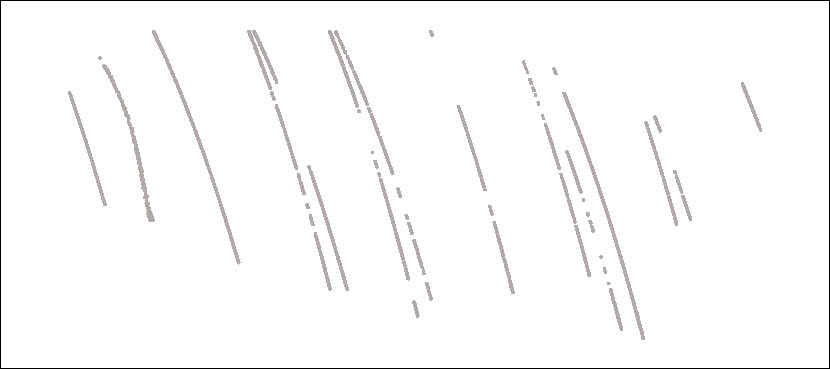
\includegraphics{figures/precompiled/datasets/oco2.pdf}
  \caption{
    Sampling 4,682 evenly spaced points from the OCO-2
    dataset, visualizing the first two features.
  }
  \label{fig:oco2}
\end{figure}

\subsubsection{OCO-2 dataset}

We also use data produced by the OCO-2 project \cite{eldering2017orbiting}
at the Jet Propulsion Laboratory, California Institute of Technology,
obtained from the OCO-2 data archive maintained at the NASA Goddard Earth
Science Data and Information Services Center which is available online at
\url{https://disc.gsfc.nasa.gov/datasets?keywords=oco2}.
OCO-2 is an orbiting satellite designed to measure atmospheric carbon dioxide.
The path an orbiting satellite takes creates characteristic
streaks in the data as shown in \cref{fig:oco2}.

We take data localized to the United States from the time
period 2017-05-16 to 2017-05-31, keeping only the features of
longitude, latitude, and time and removing any duplicates points.
We then take the first \( 2^{16} \) points and draw \( 10^3 \)
realizations from the Gaussian process with the same train test
split, kernel function, and hyperparameters as the SARCOS experiment.

As shown in \cref{fig:gp_oco2_rho}, the RMSE of
\( k \)-NN is worse than the ``KL'' baseline.
However, in every other experiment (\cref{fig:chol_rho},
\cref{fig:gp_sarcos_rho}, and \cref{fig:cg_iter}) \( k \)-NN does better
than the baseline, so neither method is strictly better than the other.
Our method, on the other hand, achieves the best accuracy
in \emph{every} numerical experiment over a wide variety
of geometries and tasks, a testament to its robustness.

\begin{figure}[t]
  \centering
  \begin{tikzpicture}[baseline, scale=0.75]
  \begin{loglogaxis}[
    grid={major},
    % title={RMSE with increasing \( \rho \)
    %   (\( N = 65536, \rho_s = 2, \lambda = 1.5 \))},
    xlabel={\( \log_{10} \) Nonzeros (nnz)},
    ylabel={\( \log_{10} \) RMSE},
    legend entries={KL, KL (agg.), \( k \)-NN, select, select (agg.)},
    legend pos={north east},
  ]
  \addplot table {figures/gp/oco2/rho_loss_KL.csv};
  \addplot table {figures/gp/oco2/rho_loss_KL_agg.csv};
  \addplot table {figures/gp/oco2/rho_loss_select-KNN.csv};
  \addplot table {figures/gp/oco2/rho_loss_select.csv};
  \addplot table {figures/gp/oco2/rho_loss_select_agg.csv};
  \end{loglogaxis}
\end{tikzpicture}
%
  \begin{tikzpicture}[baseline, scale=0.75]
  \begin{loglogaxis}[
    grid={major},
    % title={RMSE against time with increasing \( \rho \)
    %   (\( N = 65536 \rho_s = 2, \lambda = 1.5 \))},
    xlabel={\( \log_{10} \) Time (seconds)},
    % ylabel={\( \log_{10} \) RMSE},
    % legend entries={KL, KL (agg.), \( k \)-NN, select, select (agg.)},
    % legend pos={north east},
  ]
  \addplot table {figures/gp/oco2/rho_time_KL_loss.csv};
  \addplot table {figures/gp/oco2/rho_time_KL_agg_loss.csv};
  \addplot table {figures/gp/oco2/rho_time_select-KNN_loss.csv};
  \addplot table {figures/gp/oco2/rho_time_select_loss.csv};
  \addplot table {figures/gp/oco2/rho_time_select_agg_loss.csv};
  \end{loglogaxis}
\end{tikzpicture}

  \caption{
    We use a candidate set size scaling factor of \( \rho_s =
    2 \) and an aggregation parameter of \( \lambda = 1.5 \).
    The left panel shows the difference in RMSE from exact
    Gaussian process regression with varying density \( \rho \).
    The right panel shows the accuracy to computational
    time trade-off over varying \( \rho \).
  }
  \label{fig:gp_oco2_rho}
\end{figure}

\subsection{Preconditioning for conjugate gradient}
\label{subsec:cg_exp}

\begin{figure}[t]
  \centering
  \begin{tikzpicture}[baseline, scale=0.75]
  \begin{semilogyaxis}[
    grid={major},
    % title={Residual with iterations
    %   (\( N = 65536, \rho = 4, \rho_s = 2, \lambda = 1.5 \))},
    xlabel={Iterations},
    ylabel={\( \log_{10} \) Residual (\( \ell_2 \)-norm)},
    legend entries={KL, KL (agg.), select, select (agg.)},
    legend pos={north east},
  ]
  \addplot table {figures/cg/n_iter-res_KL.csv};
  \addplot table {figures/cg/n_iter-res_KL_agg.csv};
  \addplot table {figures/cg/n_iter-res_select.csv};
  \addplot table {figures/cg/n_iter-res_select_agg.csv};
  \end{semilogyaxis}
\end{tikzpicture}
%
  \begin{tikzpicture}[baseline, scale=0.75]
  \begin{axis}[
    grid={major},
    % title={Nonzero entries per column with increasing \( N \)
    %   (\( \text{iters} = 50, \rho = 4, \rho_s = 2, \lambda = 1.5 \))},
    xlabel={\( N \)},
    ylabel={Nonzeros per column},
    % legend entries={KL, KL (agg.), \( k \)-NN, select, select (agg.)},
    % legend pos={north west},
  ]
  \addplot table {figures/cg/nnz_nnz_KL.csv};
  \addplot table {figures/cg/nnz_nnz_KL_agg.csv};
  \addplot table {figures/cg/nnz_nnz_select-KNN.csv};
  \addplot table {figures/cg/nnz_nnz_select.csv};
  \addplot table {figures/cg/nnz_nnz_select_agg.csv};
  \end{axis}
\end{tikzpicture}

  \caption{
    We use the conjugate gradient preconditioned by sparse Cholesky factors to
    solve the symmetric positive-definite system \( \CM \vec{x} = \vec{y} \).
    The left panel shows iteration progress for \( N =
    2^{16} \) points and a factor density of \( \rho = 4 \).
    The right panel shows the minimum number of nonzeros
    per column for conjugate gradient to converge within
    50 iterations with an increasing number of points.
  }
  \label{fig:cg_iter}
\end{figure}

\begin{figure}[t]
  \centering
  \begin{tikzpicture}[baseline, scale=0.75]
  \begin{semilogyaxis}[
    grid={major},
    % title={Iterations with increasing \( \rho \)
    %   (\( N = 32768, \rho_s = 2, \lambda = 1.5 \))},
    xlabel={\( \rho \)},
    ylabel={\( \log_{10} \) Iterations},
    legend entries={KL, KL (agg.), select, select (agg.)},
    legend pos={north east},
  ]
  \addplot table {figures/cg/rho_iter_KL.csv};
  \addplot table {figures/cg/rho_iter_KL_agg.csv};
  \addplot table {figures/cg/rho_iter_select.csv};
  \addplot table {figures/cg/rho_iter_select_agg.csv};
  \end{semilogyaxis}
\end{tikzpicture}
%
  \begin{tikzpicture}[baseline, scale=0.75]
  \begin{semilogyaxis}[
    grid={major},
    % title={Time with increasing \( \rho \)
    %   (\( N = 32768, \rho_s = 2, \lambda = 1.5 \))},
    xlabel={\( \rho \)},
    ylabel={\( \log_{10} \) Wall-Clock Time (seconds)},
    % legend entries={KL, KL (agg.), select, select (agg.)},
    % legend pos={north west},
  ]
  \addplot table {figures/cg/rho_time_tot_KL.csv};
  \addplot table {figures/cg/rho_time_tot_KL_agg.csv};
  \addplot table {figures/cg/rho_time_tot_select.csv};
  \addplot table {figures/cg/rho_time_tot_select_agg.csv};
  \end{semilogyaxis}
\end{tikzpicture}

  \caption{
    The left panel shows how the number of iterations for the
    conjugate gradient to converge decreases with increasing
    preconditioner density \( \rho \) for \( N = 2^{16} \) points.
    The right panel shows the total wall-clock time (both to compute
    the preconditioner and to converge) with varying density.
  }
  \label{fig:cg_rho}
\end{figure}

Motivated by the equivalence of functionals like the Kaporin condition number
to the KL divergence, we investigate solving symmetric positive-definite
systems \( \CM \vec{x} = \vec{y} \) using the conjugate gradient and a sparse
Cholesky factor \( L \) as a preconditioner.
We note that from \cref{eq:kl} the KL divergence strongly
penalizes zero eigenvalues of the preconditioned matrix
\( \CM L L^{\top} \), improving its condition number.
In order to generate the covariance matrix \( \CM \) we sample up
to \( N = 2^{16} \) points uniformly at random from the unit cube
\( [0, 1]^3 \) and use a Mat{\'e}rn kernel with smoothness \( \nu
= 1/2 \) and length scale \( \ell = 1 \).
In exploratory numerical experiments, we found using higher smoothnesses
like \( \nu = 5/2 \) led to extremely poor condition numbers and
numerical instability (over thousands of iterations to converge).
Increasing length scale also worsens the
condition but to a less extreme extent.
Rather than generate a right-hand side \( \vec{y} \) directly, we first
sample a solution \( \vec{x} \sim \N(\vec{0}, \Id_N) \) and then compute
\( \vec{y} = \CM \vec{x} \) so that \( \vec{y} \) is realistically smooth.
When computing the preconditioner \( L \) by sparse Cholesky
factorization, we use a candidate set size scaling factor of \(
\rho_s = 2 \) and an aggregation parameter of \( \lambda = 1.5 \).
We then run the conjugate gradient algorithm with \( L \) as a preconditioner
until reaching a relative tolerance of \( 10^{-12} \).

As shown in \cref{fig:cg_iter}, the conditional methods converge
in half the iterations of their unconditional counterparts
and aggregation barely reduces the number of iterations.
The minimum number of nonzeros per column to converge within a constant number
of iterations (here, 50) seems to grow logarithmically with the number of
points for all methods; although the conditional methods appear near constant.

We observe a characteristic ``U'' shape for the total wall-clock time
in \cref{fig:cg_rho} from the trade-off between spending computational
time in forming the preconditioner or in conjugate gradient iterations.
Across all preconditioner densities, the aggregated variants are slower
than their non-aggregated counterparts due to barely reducing the number
of iterations while producing significantly denser factors with slower
matrix-vector products.
The time-optimal density for conditional methods is sparser than
their unconditional counterparts due to using fewer iterations at
the same sparsity and it being more expensive to select nonzeros.
It is hard to directly compare the total computational time of the methods
because simply increasing the number of iterations, e.g., by demanding better
tolerance or by using matrices with worse condition numbers, will prefer more
accurate methods even if they are slower to form the preconditioner.

\pgfplotsset{
  cycle list={
    {very thick, lightblue, style=dashed},
    {very thick, orange,    style=solid},
  }
}

\begin{figure}[t]
  \centering
  \begin{tikzpicture}[baseline, scale=0.75]
  \begin{axis}[
    grid={major},
    % title={Accuracy with increasing \( k \)
    %   (\( n = 100, m = 100, l = 1024, \nu = 1.5 \))},
    xlabel={\( k \)},
    ylabel={Accuracy (\%)},
    legend entries={\( k \)-NN, C\( k \)-NN},
    legend pos={south west},
  ]
  \addplot table {figures/mnist/k_acc_scikit-knn.csv};
  \addplot table {figures/mnist/k_acc_conditional-knn.csv};
  \end{axis}
\end{tikzpicture}
%
  \begin{tikzpicture}[baseline, scale=0.75]
  \begin{axis}[
    grid={major},
    % title={Time with increasing \( k \)
    %   (\( n = 100, m = 100, l = 1024, \nu = 1.5 \))},
    xlabel={\( k \)},
    ylabel={Time (seconds)},
    % legend entries={\( k \)-NN, C\( k \)-NN},
    % legend pos={north west},
  ]
  \addplot table {figures/mnist/k_time_scikit-knn.csv};
  \addplot table {figures/mnist/k_time_conditional-knn.csv};
  \end{axis}
\end{tikzpicture}

  \caption{
    We compare selection by Euclidean distance (\( k \)-NN) to
    conditional selection (C\( k \)-NN) in image classification.
    From the MNIST database \( N = 10^3 \) training images and \( m = 10^2
    \) testing images are randomly chosen; each test image is classified by
    the mode label of \( k \) selected images, and this process is repeated
    \( 10^2 \) times for each value of \( k \).
    (Left:) Accuracy with \( k \).
    (Right:) the time to select \( k \) points using C\( k \)-NN seems to
    scale linearly with \( k \) although it is quadratic asymptotically;
    possibly resulting from applying highly optimized BLAS operations to
    relatively small matrices.
  }
  \label{fig:mnist}
\end{figure}

\subsection{k-nearest neighbors selection}
\label{subsec:knn_exp}

We compare \( k \)-nearest neighbors (\( k \)-NN) to our selection
algorithm from \cref{subsec:greedy_select}, which we call conditional
\( k \)-nearest neighbors (C\( k \)-NN), in the following toy example
performing image classification.
From the MNIST database of handwritten digits
\cite{lecun1998gradientbased}, we randomly select \( N =
10^3 \) training images and \( m = 10^2 \) testing images.
We classify a test image by selecting \( k \) training
images and taking the mode label of those images.
For \( k \)-NN, we use the Euclidean distance and for C\(
k \)-NN, we use a Mat{\'e}rn kernel with smoothness \( \nu
= 3/2 \) and length scale \( \ell = 2^{10} \).
Accuracy is the percentage of test images classified correctly.

The accuracy of both methods decreases linearly with
increasing \( k \) as shown in \cref{fig:mnist}.
We hypothesize that nearby images are more likely to
have the same label, so selecting more points increases
the influence of further, differently labeled images.
C\( k \)-NN remains more accurate than \( k \)-NN for every \( k >
2 \), suggesting it consistently selects more informative images.
We emphasize that conditioning alone causes the difference in accuracy:
unconditional covariance decays monotonically with distance.

\pgfplotsset{
  cycle list={
    {very thick, silver,    style=densely dotted},
    {very thick, lightblue, style=dashed},
    {very thick, seagreen,  style=dashdotted},
    {very thick, orange,    style=solid},
  }
}

\begin{figure}[t]
  \centering
  \begin{tikzpicture}
  \begin{axis}[
    width={0.8\linewidth},
    grid={major},
    title={Accuracy with increasing \( N \)
    (\( s = 32 \))},
    xlabel={\( N \)},
    ylabel={Accuracy (IOU)},
    legend entries={cknn, knn, corr, random},
    legend pos={south west},
  ]
  \addplot [orange]    table {figures/recover/n_score_cknn.csv};
  \addplot [lightblue] table {figures/recover/n_score_knn.csv};
  \addplot [seagreen]  table {figures/recover/n_score_corr.csv};
  \addplot [silver]    table {figures/recover/n_score_random.csv};
  \end{axis}
\end{tikzpicture}
%
  \begin{tikzpicture}[baseline, scale=0.75]
  \begin{axis}[
    grid={major},
    % title={Accuracy with increasing \( s \)
    %   (\( N = 256 \))},
    xlabel={\( s \)},
    % ylabel={Accuracy (IOU)},
    legend entries={rand., \( k \)-NN, corr., C\( k \)-NN},
    legend pos={south east},
    ymin=0, ymax=1.1,
  ]
  \addplot table {figures/recover/s_score_random.csv};
  \addplot table {figures/recover/s_score_knn.csv};
  \addplot table {figures/recover/s_score_corr.csv};
  \addplot table {figures/recover/s_score_cknn.csv};
  \end{axis}
\end{tikzpicture}

  \caption{
    We attempt to recover a sparse Cholesky factor \(
    L \) of the precision matrix \( Q = L L^{\top} \).
    ``C\( k \)-NN'' minimizes the conditional variance of the target
    (diagonal) entry, ``corr.'' maximizes correlation with the target,
    ``\( k \)-NN'' maximizes covariance with the target, and ``rand.''
    samples entries uniformly at random.
    All methods achieve their best accuracy given \( Q \) except
    C\( k \)-NN which is given the covariance matrix \( Q^{-1} \).
    (Left:) Varying the size of \( L \), fixed density \( s = 2^5 \).
    (Right:) Varying \( s \), fixed size \( N = 2^8 \).
    Accuracy starts to improve from the factor nearing fully dense.
  }
  \label{fig:recover_acc}
\end{figure}

\begin{figure}[t]
  \centering
  \begin{tikzpicture}[baseline, scale=0.75]
  \begin{axis}[
    grid={major},
    % title={Accuracy with increasing \( \sigma^2 \)
    %   (\( N = 1024, s = 32 \))},
    % 0.05 shows up as \( 5 \cdot 10^{-2} \), suppress exponential
    every tick label/.append style={/pgf/number format/fixed},
    xlabel={\( \var \)},
    ylabel={Accuracy (IOU)},
    legend entries={rand., \( k \)-NN, corr., C\( k \)-NN},
    legend pos={north east},
    legend style={nodes={scale=0.85, transform shape}},
    ymin=0, ymax=1.1,
  ]
  \addplot+ [mark=triangle*] table {figures/recover/noise_score_random.csv};
  \addplot+ [mark=*]         table {figures/recover/noise_score_knn.csv};
  \addplot+ [mark=o]         table {figures/recover/noise_score_corr.csv};
  \addplot+ [mark=square*]   table {figures/recover/noise_score_cknn.csv};
  \end{axis}
\end{tikzpicture}
%
  \begin{tikzpicture}[baseline, scale=0.75]
  \begin{axis}[
    grid={major},
    % title={Accuracy with increasing \( s \)
    %   (\( N = 256 \))},
    xlabel={\( s \)},
    % ylabel={Accuracy (IOU)},
    legend entries={\( \var = 0.00 \), \( \var = 0.01 \),
      \( \var = 0.10 \), \( \var = 0.20 \)},
    legend pos={south east}
  ]
  \addplot [very thick, orange, style=solid]
    table {figures/recover/noise-s_score_cknn-0.00.csv};
  \addplot [very thick, orange, style=dashed]
    table {figures/recover/noise-s_score_cknn-0.01.csv};
  \addplot [very thick, orange, style=dotted]
    table {figures/recover/noise-s_score_cknn-0.10.csv};
  \addplot [very thick, orange, style=dashdotted]
    table {figures/recover/noise-s_score_cknn-0.20.csv};
  \end{axis}
\end{tikzpicture}

  \caption{
    We add noise sampled i.i.d. from \( \N(0, \var)
    \) to the measurements \( Q \).
    The left panel shows accuracy with varying noise for \( N
    = 2^{10} \) columns and \( s = 2^5 \) nonzeros per column.
    The right panel shows accuracy for the C\( k \)-NN method at
    various noise levels for \( N = 2^8 \) and varying \( s \).
  }
  \label{fig:recover_noise}
\end{figure}

\subsection{Recovery of sparse Cholesky factors}
\label{subsec:recover_exp}

Motivated by the similarity of the selection algorithm to orthogonal matching
pursuit \cite{tropp2007signal}, we attempt to recover an \textit{a priori}
sparse Cholesky factor \( L \) from its precision matrix \( Q = L L^{\top} \).
To generate the nonzero entries of \( L \), for each column
we pick \( s \) lower triangular indices uniformly at
random and sample their values i.i.d. from \( \N(0, 1) \).
We fill \( L \)'s diagonal with a ``large'' positive
value 10 to ensure \( Q \) is well-conditioned.
The selection algorithm is given \( s \) and either \(
Q \) or the covariance matrix \( Q^{-1} \) depending on
which results in higher accuracy in reconstructing \( L \).
For a recovered sparsity pattern \( X \) and ground truth \( Y \) we report
\( \card{X \cap Y}/\card{X \cup Y} \), the intersection over union (IOU).
Using the KL divergence \cref{eq:L_obj} of the recovered
Cholesky factor seems mostly equivalent to IOU.

As shown in \cref{fig:recover_acc}, C\( k \)-NN maintains a near-perfect
recovery accuracy much higher than the unconditional baselines.
In the setting of noisy measurements, noise sampled i.i.d from
\( \N(0, \var) \) is symmetrically added to each entry of \( Q
\) (\( Q_{i, j} \) receives the same noise as \( Q_{j, i} \)).
Accuracy degrades with increasing noise for all methods, but C\( k \)-NN
is the most sensitive to noise as is shown in \cref{fig:recover_noise}.
At high enough levels of noise \( Q \) can lose
positive-definiteness, causing C\( k \)-NN to break down entirely.

% An important setting where \( Q \) (and possibly \( L \)) are known
% to be \textit{a priori} sparse is when solving Laplacian systems.
% In exploratory numerical experiments we found that the factors
% generated by our method were unreasonably dense compared the sparsity
% of the Laplacian matrix, a manifestation of \emph{fill-in}.
% We comment that our method is designed for \emph{dense} kernel matrices
% resulting from a set of points and a ``well-behaved'' kernel function.
% For solving sparse Laplacian systems, a method designed
% to exploit the sparsity and graph structure of Laplacian
% matrices like \cite{kyng2016approximate} is more appropriate.

\section{Comparisons and conclusion}
\label{sec:conclusion}

We briefly compare our method to prior works.

\subsection{Comparison to other methods}
\label{subsec:compare}

\paragraph{Local approximate Gaussian process (laGP)}

Our conditional variance objective for point selection \cref{eq:obj_gp} was
first described in \cite{cohn1996neural} for optimal experimental design,
and has subsequently been named the active learning Cohn (ALC) technique.
\cite{gramacy2014local} and the follow-up works \cite{gramacy2015speeding,
sun2019emulating} apply ALC to directed Gaussian process inference, yielding
an algorithm equivalent to ours described in \cref{subsec:greedy_select} for
a single point of interest.
We note that their definition of conditional variance in Equation (5) is
analogous to our \cref{eq:cond_cov}, equating their conditional variance
objective in Equation (8) to our \cref{eq:obj_gp} (the connection is
explicitly stated in SM\S4's Equation (SM.22)).
They also update the precision by the blocked
equations in SM\S1 like our \cref{app:prec_insert}.

For inference at multiple points of interest, \cite{gramacy2014local} suggests
direct parallelization of the single-target algorithm over each target.
They mention that the \texttt{laGP} function in their
\texttt{R} package jointly considers multiple target
points, but without providing details on this procedure.
\cite{sun2019emulating} proposes a ``joint'' or ``path'' ALC by taking
the average reduction in posterior variance over target points.
Instead, we generalize ALC to multiple prediction points through
their posterior log determinant \cref{eq:greedy_mult} and provide
an explicit algorithm described in \cref{subsec:mult_select}.
In addition, integration of the algorithm into Cholesky factorization
(\cref{sec:chol_select}) provides a global approximation of the Gaussian
process (\cref{subsec:gp_exp}) beyond directed local approximation.

\paragraph{Orthogonal matching pursuit (OMP)}

Our selection algorithm can be viewed as the covariance equivalent
of the sparse signal recovery algorithm orthogonal matching
pursuit (OMP) \cite{tropp2007signal, tropp2006algorithms}.
OMP measures the approximation of a target signal by its residual after
orthogonal projection onto the subspace of chosen training signals,
which is efficiently calculated by maintaining a QR factorization.
In contrast, our selection algorithm uses a kernel function to evaluate inner
products, so orthogonalization becomes conditioning, the residual norm
becomes variance, and the QR factorization becomes a Cholesky factorization.
A major difference from OMP is that the computational time of conditioning
dominates that of evaluating the kernel function since the feature space
is relatively low-dimensional (often 2 or 3 in spatial statistics).

\paragraph{Sparse Cholesky factorization}

Our sparse Cholesky factorization algorithm proposed in
\cref{sec:chol_select} relies heavily on the KL-minimization framework of
\cite{schafer2021sparse} and is similar to \cite{kang2021correlationbased}.
We comment that using \( k \)-nearest neighbors to select the
sparsity set instead of our conditional selection algorithms
essentially recovers \cite{schafer2021sparse} and that using
the correlation objective \cref{eq:obj_gp} without conditioning
on selected points recovers \cite{kang2021correlationbased}.

\subsection{Conclusion}

In this work, we develop an algorithm for directed Gaussian process
regression which greedily selects training points that maximize
mutual information with a target point, conditional on all points
previously selected to avoid redundancy.
We show that using conditional selection to pick the sparsity pattern of
sparse approximate Cholesky factors of precision matrices significantly
improves accuracy and performance in downstream tasks compared to selection
by nearest neighbors.
Single-target conditional selection is computationally efficient and can
be extended to the settings of multiple-target and partial conditioning
corresponding to aggregated (or supernodal) Cholesky factorization.
Finally, global selection gives a principled way of
distributing nonzeros over columns of the Cholesky factor.
We support these claims through extensive numerical
experimentation in a variety of problems.

\section*{Acknowledgments}
\todo{add more funding information}
This research was supported in part by research cyberinfrastructure resources
and services provided by the Partnership for an Advanced Computing Environment
(PACE) at the Georgia Institute of Technology, Atlanta, Georgia, USA.
HO acknowledges support from the Air Force Office of Scientific Research under
MURI award number FA9550-20-1-0358 (Machine Learning and Physics-Based Modeling
and Simulation) and the Department of Energy from the Department of Energy under award number DE-SC0023163 (SEA-CROGS: Scalable, Efficient and Accelerated Causal Reasoning Operators, Graphs and Spikes for Earth and Embedded Systems).

\bibliographystyle{siamplain}
\bibliography{references}

\newpage

\appendix

\todo{add proofs, if any, in appendix}

\section{Derivations in KL-minimization}

\subsection{KL divergence of optimal factor}
\label{app:kl_L}

% In \cref{subsec:kl}, we wish to compute the KL divergence between the
% covariance matrix \( \CM \) and the optimal sparse approximate Cholesky
% factor \( L \) computed from the closed-form expression \cref{eq:L_col}.
\begin{proof}[Proof of Equation \cref{eq:obj_chol}]
  From the closed-form expression for the KL divergence in
  \cref{eq:kl} and defining \( \Delta \defeq 2 \KL*{\N(\vec{0},
  \CM)}{\N(\vec{0}, (L L^{\top})^{-1})} \) for brevity of notation,
  \begin{align}
    \label{eq:kl_L}
    \Delta &= \trace(L L^{\top} \CM) - \logdet(L L^{\top}) - \logdet(\CM) - N.
    \shortintertext{
      Focusing on the term \( \trace(L L^{\top} \CM) = \trace(L^{\top} \CM L)
      \) by the cyclic property of trace and using the sparsity of \( L \) by
      plugging in the definition \cref{eq:L_col} for each column \( L_{s_i, i}
      \),
    }
    \trace(L^{\top} \CM L) &= \sum_{i = 1}^N
      L_{s_i, i}^{\top} \CM_{s_i, s_i} L_{s_i, i} \\
    &= \sum_{i = 1}^N
      \left (
        \frac{\left ( \CM_{s_i, s_i}^{-1} \vec{e}_1 \right )^{\top}}
          {\sqrt{\vec{e}_1^{\top} \CM_{s_i, s_i}^{-1} \vec{e}_1}}
      \right )
      \CM_{s_i, s_i}
      \left (
        \frac{\CM_{s_i, s_i}^{-1} \vec{e}_1}
          {\sqrt{\vec{e}_1^{\top} \CM_{s_i, s_i}^{-1} \vec{e}_1}}
      \right ) \\
    &= \sum_{i = 1}^N
      \frac{\vec{e}_1^{\top} \CM_{s_i, s_i}^{-1}
            \CM_{s_i, s_i} \CM_{s_i, s_i}^{-1}
            \vec{e}_1}{\vec{e}_1^{\top} \CM_{s_i, s_i}^{-1} \vec{e}_1}
    = \sum_{i = 1}^N 1 = N,
    \shortintertext{
      exactly the constraint \( \diag(L^{\top} \CM L) = 1 \)
      from \cref{subsec:vecchia}.
      Substituting back into \cref{eq:kl_L},
    }
    \Delta &= -\logdet(L L^{\top}) - \logdet(\CM).
    \shortintertext{
      Computing the log determinant of a triangular matrix as
      the sum of the log of its diagonal entries and plugging in
      the definition \cref{eq:L_col} for the diagonal entries,
    }
    &= -\sum_{i = 1}^N
      \left [ \log(\vec{e}_1^{\top} \CM_{s_i, s_i}^{-1} \vec{e}_1) \right ]
      - \logdet(\CM) \\
    &= \sum_{i = 1}^N
      \left [
        \log
        \left (
          (\vec{e}_1^{\top} \CM_{s_i, s_i}^{-1} \vec{e}_1)^{-1}
        \right )
      \right ]
      - \logdet(\CM).
    \shortintertext{
      Now we use that conditioning in
      covariance is marginalization in precision,
    }
    \label{eq:inverse_cond}
    \CM_{1, 1 \mid 2} &= \left ( \CM^{-1} \right )_{1, 1}^{-1}
    \qquad \qquad \text{for }
    \CM =
      \begin{pmatrix}
        \CM_{1, 1} & \CM_{1, 2} \\
        \CM_{2, 1} & \CM_{2, 2}
      \end{pmatrix}.
    \shortintertext{
      Transforming the marginalization \( (\vec{e}_1^{\top} \CM_{s_i, s_i}^{-1}
      \vec{e}_1)^{-1} = \left (\CM_{s_i, s_i}^{-1} \right )_{1, 1}^{-1} =
      \CM_{i, i \mid s_i \setminus \{ i \}} \) by \cref{eq:inverse_cond},
    }
    \Delta &= \sum_{i = 1}^N
      \left [
        \log \left ( \CM_{i, i \mid s_i \setminus \{ i \}} \right )
      \right ]
      - \logdet(\CM). \\
    \shortintertext{Now we use the chain rule of log determinants,
      using the same blocking as \cref{eq:inverse_cond},}
    \label{eq:det_chain}
    \logdet(\CM) &= \logdet(\CM_{1, 1}) + \logdet(\CM_{2, 2 \mid 1}). \\
    \shortintertext{
      Repeatedly expanding the log determinant by
      \cref{eq:det_chain}, working from back to front,
    }
    \Delta &= \sum_{i = 1}^N
        \log \left ( \CM_{i, i \mid s_i \setminus \{ i \}} \right ) -
      \sum_{i = 1}^N
        \log \left ( \CM_{i, i \mid i + 1:} \right ) \\
    &= \sum_{i = 1}^N
      \left [
        \log \left ( \CM_{i, i \mid s_i \setminus \{ i \}} \right ) -
        \log \left ( \CM_{i, i \mid i + 1:} \right )
      \right ].
  \end{align}
\end{proof}

\subsection{Aggregated KL divergence}
\label{app:kl_agg}

% In the aggregated Cholesky factorization setting of
% \cref{subsec:aggregated}, we have indices \( \tilde{i} = \{i_1,
% \dotsc, i_m \} \) such that \( i_1 \succ \dotsb \succ i_m \).
% Let the selected entries be \( \tilde{s} \); we assume every selected entry is
% after (w.r.t \( \succ \)) every index in \( \tilde{i} \) so that the sparsity
% pattern for the \( k \)th column is \( s_k = \tilde{s} \cup \{ j \in \tilde{i}
% : j \succeq k \} \).
\begin{proof}[Proof of Equation \cref{eq:obj_mult}]
  The KL divergence \cref{eq:obj_chol}
  restricted to the group \( \tilde{i} \) is
  \begin{align}
    \sum_{i \in \tilde{i}} \log(\CM_{i \mid s_i \setminus \{ i \} }) &=
      \log(\CM_{i_1 \mid \tilde{s}}) +
      \log(\CM_{i_2 \mid \tilde{s} \cup \{ i_1 \}}) + \dotsb +
      \log(\CM_{i_m \mid \tilde{s} \cup \tilde{i}}) \\
    \shortintertext{
      where we write \( \CM_j \defeq \CM_{j, j} \).
      Combining the first two terms by the chain rule \cref{eq:det_chain},
    }
    &= \logdet(\CM_{\{ i_1, i_2 \} \mid \tilde{s}}) +
      \log(\CM_{i_3 \mid \tilde{s} \cup \{ i_1, i_2 \}}) + \dotsb +
      \log(\CM_{i_m \mid \tilde{s} \cup \tilde{i}}). \\
    \shortintertext{
      Proceeding by induction, we are able to
      reduce the entire sum to the single term
    }
    &= \logdet(\CM_{\tilde{i}, \tilde{i} \mid \tilde{s}}).
  \end{align}
\end{proof}

\subsection{Partial KL divergence}
\label{app:partial}

\begin{figure}[t]
  \centering
  
\begin{tikzpicture}[scale=3]
  % left matrix
  \fill[lightsilver, opacity=1.0]   (0,        0) rectangle (1, -1);
  \fill[lightblue,   opacity=0.5]   (0,    -0.75) rectangle (0.75, -1);
  \fill[lightblue,   opacity=0.5]   (0.75,     0) rectangle (1, -0.75);
  \fill[lightblue,   opacity=1.0]   (0.75, -0.75) rectangle (1, -1);

  % equals sign
  \node at (1.25, -0.5) {\Huge \textcolor{darksilver}{$=$}};

  % lower triangle
  \fill[lightsilver]
    (1.5, -1) -- (2.5, -1) -- (1.5, 0) -- cycle;
  \fill[lightblue]
    (1.5, -1) -- (2.5, -1) -- (2.25, -0.75) -- (1.5, -0.75) -- cycle;

  % times
  \node at (2.05, -0.5) {\Huge \textcolor{darksilver}{$\cdot$}};

  % upper triangle
  \fill[lightsilver]
    (2.6, -1) -- (2.6, 0) -- (1.6, 0) -- cycle;
  \fill[lightblue]
    (2.6, -1) -- (2.6, 0) -- (2.35, 0) -- (2.35, -0.75) -- cycle;
\end{tikzpicture}

  \caption{
    Illustration of the Cholesky factorization of
    a partially conditioned covariance matrix.
    Here \textcolor{darksilver}{grey} denotes fully unconditional,
    \textcolor{darklightblue}{blue} denotes fully conditional, and the
    \textcolor{silver!50!lightblue}{mixed color} denotes interaction
    between the two.
    Surprisingly, such a matrix factors into a ``pure'' Cholesky
    factor by ``gluing'' the prefix of the fully unconditional
    factor with the suffix of the fully conditional factor.
  }
  \label{fig:partial_factor}
\end{figure}

% In the setting of \cref{subsubsec:partial}, we have the
% Gaussian random variables \( \vec{y} = [y_1, \dotsc, y_m]^{\top} \)
% corresponding to ordered column indices \( i_1 \succ \dotsb \succ
% i_m \) grouped in \( \tilde{i} \).
% We select an index \( k \) that conditions all but the first \( p \)
% variables and wish to compute the covariance \( \Cov[\vec{y}_{\parallel
% k}] \) of the updated variables \( \vec{y}_{\parallel k} \).
\begin{proof}[Proof of Equation \cref{eq:partial_kl}]
  The original variables \( \vec{y} \) have joint density multivariate
  Gaussian, \( \vec{y} \sim \N(\vec{0}, \CM) \) for some covariance matrix
  \( \CM \) so the fully conditional variables \( \vec{y}_{\mid k} \) have
  posterior distribution from \cref{eq:cond_mean} and \cref{eq:cond_cov},
  \( \vec{y}_{\mid k} \sim \N(\vec{\mean}, \CM_{:, : \mid k}) \) for some
  posterior mean \( \vec{\mean} \).
  The covariance of unconditioned \( y_i \) and \( y_j \) is \( \CM_{i,
  j} \) by definition; similarly, the covariance of conditioned \(
  y_{i \mid k} \) and \( y_{j \mid k} \) is \( \CM_{i, j \mid k} \).
  We must compute the covariance between unconditioned
  \( y_i \) and conditioned \( y_{j \mid k} \).
  Let \( L = \chol(\CM) \) and \( L' = \chol(\CM_{:, : \mid k}) \)
  so that \( \vec{y} = L \vec{z} \) for \( \vec{z} \sim \N(\vec{0},
  \Id) \) and \( \vec{y}_{\mid k} = L' \vec{z} + \vec{\mean} \).
  By the definition of covariance,
  \begin{align}
    \Cov[y_i, y_{j \mid k}] &=
      \E[(y_i - \E[y_i])(y_{j \mid k} - \E[y_{j \mid k}])]
      = \E[(L_i \vec{z}) ({L'}_j \vec{z} + \mu_j - \mu_j)] \\
    &= \E[(L_{i, 1} z_1 + \dotsb + L_{i, m} z_m)
          ({L'}_{j, 1} z_1 + \dotsb + {L'}_{j, m} z_m)].
    \shortintertext{
      For \( i \neq j \), \( \E[z_i z_j] = \E[z_i] \E[z_j] = 0 \)
      since \( z_i \) is independent of \( z_j \) and has mean 0,
    }
    &= L_{i, 1} {L'}_{j, 1} \E[z_1^2] + \dotsb +
       L_{i, m} {L'}_{j, m} \E[z_m^2].
    \shortintertext{
      For any \( i \), \( \E[z_i^2] = \Var[z_i] + \E[z_i]^2 = 1 + 0 = 1 \),
    }
    &= L_{i, 1} {L'}_{j, 1} + \dotsb + L_{i, m} {L'}_{j, m} = L_i^{\top} {L'}_j.
    \shortintertext{
      Thus, the new covariance matrix factors into
      two Cholesky factors ``glued'' together,
    }
    \Cov[\vec{y}_{\parallel k}] &=
    \begin{pmatrix}
      L_{:p} L_{:p}^{\top} &
      L_{:p} {L'}_{p + 1:}^{\top} \\
      {L'}_{p + 1:} L_{:p}^{\top} &
      {L'}_{p + 1:} {L'}_{p + 1:}^{\top}
    \end{pmatrix} =
    \begin{pmatrix}
      L_{:p} \\
      {L'}_{p + 1:}
    \end{pmatrix}
    \begin{pmatrix}
      L_{:p} \\
      {L'}_{p + 1:}
    \end{pmatrix}^{\top}
  \end{align}
  which is illustrated in \cref{fig:partial_factor}.
  Armed with this representation, we equate the log determinant of \(
  \CM_{\tilde{i}, \tilde{i} \parallel k} \defeq \Cov[\vec{y}_{\parallel
  k}] \) to the KL divergence in \cref{eq:obj_chol}.
  Recalling that the determinant of a triangular
  matrix is the product of its diagonal entries,
  \begin{align}
    \nonumber
    \frac{1}{2} \logdet(\CM_{\tilde{i}, \tilde{i} \parallel k}) &=
    \underbrace{
      \log(L_{1, 1}) + \dotsb + \log(L_{p, p})
    }_{\text{the same}} +
    \underbrace{
      \log({L'}_{p + 1, p + 1}) + \dotsb + \log({L'}_{m, m})
    }_{\text{conditioned}}.
  \end{align}
  Comparing to the KL divergence \cref{eq:obj_chol} and
  recalling that \( k \) is added to \( s_i \) if \( i > p \),
  \begin{align}
    \sum_{i = 1}^m \log \left ( \CM_{i, i \mid s_i \setminus \{ i \}} \right )
    = &\underbrace{
        \log \left ( \CM_{1, 1 \mid s_1 \setminus \{ 1 \}} \right ) + \dotsb +
        \log \left ( \CM_{p, p \mid s_p \setminus \{ p \}} \right )
      }_\text{the same} + \\
    \nonumber
    &\underbrace{
      \log \left (
        \CM_{p + 1, p + 1 \mid s_{p + 1} \setminus \{ p + 1 \}}
      \right ) + \dotsb +
      \log \left ( \CM_{m, m \mid s_m \setminus \{ m \}} \right )
    }_\text{conditioned}.
    \shortintertext{
      Since \( L_{i, i} \) (and \( {L'}_{i, i} \)) is the square root
      of the posterior variance of the \( i \)th variable from the
      statistical perspective in \cref{eq:chol}, we have \( 2 \log(L_{i,
      i}) = \log(\CM_{i, i \mid s_i \setminus \{ i \}}) \) and so
    }
    \logdet(\CM_{\tilde{i}, \tilde{i} \parallel k}) &=
      \sum_{i = 1}^m
        \log \left ( \CM_{i, i \mid s_i \setminus \{ i \}} \right ).
  \end{align}
\end{proof}

\end{document}
